 

\setchapterpreamble[ur]{%
\dictum[D.~Adams~\cite{adams2002salmon}]{%
Anything that is in the world when you’re born is normal and ordinary and is just a natural part of the way the world works.

Anything that's invented between when you’re fifteen and thirty-five is new and exciting and revolutionary and you can probably get a career in it.

Anything invented after you're thirty-five is against the natural order of things.%
}%
\vspace*{2cm}}



%%%%%%%%%%%%%%%%%%%%%%%%%%%%%%%%%%%%%%%%%%%%%%%%%%%%%%%%%%%%
\chapter{Better Higgs measurements through information geometry}
\label{chapter:information}
%%%%%%%%%%%%%%%%%%%%%%%%%%%%%%%%%%%%%%%%%%%%%%%%%%%%%%%%%%%%

\firstword{W}{ith the results of the last chapter,} we rest assured
that many potential signatures of new physics in Higgs observables can
be parametrised by dimension-six operators. The next question is how
the corresponding Wilson coefficients can be measured as precisely as
possible. In this chapter we develop statistical tools based on
information geometry that can help to optimise such measurements.

After an introduction in \autoref{sec:information_intro}, in
\autoref{sec:information_formalism} we summarize the statistics of the
measurement process, define the Fisher information, and discuss what
constitutes an optimal measurement. In
\autoref{sec:information_madfisher} we apply these general ideas to
LHC physics and develop an algorithm to calculate the Fisher
information in particle physics processes. We also discuss some
aspects of information geometry particular to effective field
theories. In \autoref{sec:information_application_even} we use our
formalism to understand how $CP$-even dimension-six operators can be
measured in a range of Higgs channels.
Section~\autoref{sec:information_application_odd} focusses on the
measurement of $CP$ violation. We demonstrate how our approach can be
extended to describe systematic uncertainties, and link it to other
statistical tools, in \autoref{sec:information_extensions}, and
finally give our conclusions in \autoref{sec:information_conclusions}.

Most of the research presented in this chapter was previously
published in Reference~\cite{Brehmer:2016nyr}. The results and their
presentation, including nearly all plots and tables as well as part of
the text, are identical to that in this article. The exception is
\autoref{sec:information_application_odd}, which is based on ongoing
and yet unpublished work~\cite{Brehmer:CPV_information}.



%%%%%%%%%%%%%%%%%%%%%%%%%%%%%%%%%%%%%%%%%%%%%%%%%%%%%%%%%%%%
\section{Introduction}
\label{sec:information_intro}
%%%%%%%%%%%%%%%%%%%%%%%%%%%%%%%%%%%%%%%%%%%%%%%%%%%%%%%%%%%%

Having established that the dimension-six operators of the linear
Higgs effective theory capture the indirect signatures of many
scenarios of new physics, we now analyse how its parameters, the
Wilson coefficients $f_i/\Lambda^2$, can be measured most efficiently
at the LHC. This is a highly non-trivial problem for two reasons:
first, the Higgs properties form a high-dimensional parameter
  space. In \autoref{sec:foundations_heft_operators} we showed that
even after removing redundant operators and generously neglecting
those with tight limits from electroweak precision measurements or
flavour constraints, we are left with thirteen dimension-six operators
relevant for Higgs physics. The Higgs-gauge interactions, for
instance, are affected by seven of these operators, equivalent to a
range of different kinematic structures or forms of momentum
dependence. The second challenge comes from the complicated
  kinematics of some of the Higgs production channels and decay
modes. For example, Higgs production in weak boson fusion with a decay
$h \to W^+W^- \to (\ell^+ \nu) (\ell^- \overbar{\nu})$ is a $2 \to 6$
process even at parton level, and only made more complicated by
additional QCD radiation. Such a high-dimensional phase space defines
a large number of kinematic observables, and it is often not obvious
which of them carry information on the theory parameters of
interest. The relation between the high-dimensional parameter space
and the potentially high-dimensional phase space is (at parton level)
encoded in the amplitudes or Feynman diagrams, of which there can
easily be hundreds for a given process.

\emph{Traditional analysis methods} typically begin with simple
selection cuts on standard kinematic observables such as energies,
momenta, angles, or invariant masses. This is often followed by the
estimation of background contributions with a mixture of simulational
and data-driven methods. The final statistical analysis typically
relies on total event counts or on histograms of kinematic
observables.  These techniques are very intuitive and all steps are
transparent. They they work well for simple signatures, such as a
resonance peak on top of a smooth background, as in the discovery of
the $gg \to h \to \gamma \gamma$
signal~\cite{Aad:2012tfa,Chatrchyan:2012xdj}. This approach requires a
careful tailoring of the strategy to each question, and does not scale
well with the complexity of the theory questions or the kinematics of
the processes.

At the other end of the spectrum, the LHC collaborations increasingly
rely on measurement strategies based on high-level statistical
tools~\cite{cranmer:nips2016}. Some of them are based on the structure
of the \emph{matrix elements} contributing to the process. In the
matrix element method~\cite{Kondo:1988yd, Abazov:2004cs, Gao:2010qx,
  Alwall:2010cq, Avery:2012um, Andersen:2012kn, Campbell:2013hz,
  Artoisenet:2013vfa, Martini:2015fsa, Gritsan:2016hjl}, the
differential cross section expected from a given model hypothesis at a
specific phase-space point, or the ratio of two such expected rates,
is directly used as an observable. The detector response is estimated
by convuluting this expression with suitable transfer
functions. Shower deconstruction~\cite{Soper:2011cr, Soper:2012pb} and
even deconstruction~\cite{Soper:2014rya} extend this concept to the
parton shower to take into account the information encoded in jet
substructure. Optimal observables~\cite{Atwood:1991ka, Davier:1992nw,
  Diehl:1993br} apply the same idea to the measurement of a small
theory parameter. All these tools intrinsically make full use of the
information encoded in the underlying field theories, but rely on an
approximate description of the detector systems. They are particularly
useful in channels with not too many particles in the final state that
can be reconstructed precisely. Large final-state multiplicities
require a high-dimensional integration and is computationally
expensive. Finally, matrix-element-based tools generally rely on the
comparison of two discrete hypotheses or for the measurement of one
model parameter, \ie one direction in theory space. Applying these
methods to high-dimensional theory spaces such as Higgs effective
field theory often requires a discretization of the theory space,
which can be computationally expensive, and care has to be taken to
avoid dependencies on EFT basis choices.

A second class of statistical tools falls under the category of
\emph{likelihood-free inference}~\cite{cranmer:nips2016}. They are
mostly based on (supervised) machine learning techniques:
sophisticated interpolation techniques, such as boosted decision trees
and neural networks, are used to describe patterns in a set of
training samples. This approach is agnostic about the amplitudes
describing a process. The methods with which the input samples are
generated is irrelevant. Unlike simple likelihood-based methods, these
samples can be based on data as well as complicated Monte-Carlo
simulations with a parton shower and full detector simulation. New
technologies are developed at an impressive
pace~\cite{Cranmer:2015bka, Louppe:2016ylz, Louppe:2016aov,
  Cranmer:2016lzt, Baldi:2016fzo}. These tools are applied to problems
at all steps of the analysis process, ranging from
tracking~\cite{Brehmer:ghost_probability} over the analysis of jet
substructure~\cite{Cogan:2014oua, Baldi:2014pta, deOliveira:2015xxd,
  Almeida:2015jua, Baldi:2016fql, Guest:2016iqz, Komiske:2016rsd,
  Kasieczka:2017nvn, Louppe:2017ipp} to the discrimination between
signal and background hypotheses~\cite{Baldi:2014kfa, Searcy:2015apa,
  Santos:2016kno, Alves:2016htj} and finally to the statistical
testing of model hypotheses~\cite{Buckley:2011kc, Bornhauser:2013aya,
  Bechtle:2017vyu}. For complicated problems, multivariate tools often
outperform traditional approaches. However, their inner structure is
often convoluted and not necessarily very unintuitive; and it is not
always clear which physical structures these ``black boxes'' are
sensitive to.

\newparagraph
%
With these wide range capabilities, it is increasingly important that
we can understand and characterise the information contained in
particle physics processes. The design of event selections and
analysis strategies requires clearly defined guidelines. We present an
approach to these problems based on information
geometry~\cite{efron1975, amari1982}. It offers tools that are
intrinsically designed for continous parameter spaces of arbitrary
dimensionality, independent of basis choices and without the need for
any discretization of the model hypothesis.

The central object in our approach is the \emph{Fisher information}
matrix. According to the Cram\'er-Rao bound~\cite{Rao:1945,
  Cramer:1946}, it quantifies the maximum knowledge on
theory parameters that we can derive in a measurement, independent of
the analysis strategy. This allows us to calculate the best possible
precision with which theory parameters can be measured with any
multivariate black-box analysis. Also, the Fisher information defines
a metric in the space of theory parameters. This provides an intuitive
geometric interpretation for the discrimination power of an
experiment. From a practical perspective, it gives us a handle on the
linearisation of observables in terms of new physics parameters, as we
demonstrate in the next section.

Two objects are particularly interesting for LHC physics.  First, the
distribution of the differential information over phase space defines
the relevance of different phase-space regions for an analysis and
should motivate the design of event selections. Second, we can
calculate the information contained in individual kinematic
observables and compare it to the full Fisher information. This
determines the most important observables and allows us to compare the
power of traditional histogram-based analyses to that of modern
multivariate tools.

We develop an algorithm, which we call \toolfont{MadFisher}, that can
calculate the Fisher information for arbitrary perturbative
particle-physics processes based on Monte-Carlo methods. We can
calculate the quantities outlined above, each designed to answer
different practical questions:
%
\begin{itemize}
\item \emph{full Fisher information}: what is the maximum precision
  with which continous model parameters can be measured in a process?
    %
\item \emph{differential Fisher information}: how is the information
  on model parameters distributed over phase space?
    %
\item \emph{information in distributions}: how well can we measure
  model parameters based on individual kinematic observables, rather
  than the information in the full high-dimensional phase space?
    %
\item \emph{global geometry}: which role do non-linear terms in the
  theory parameters play?
\end{itemize}

\newparagraph
%
As a first application we calculate the information on $CP$-even
dimension-six operators in WBF Higgs production with a decay into tau
pairs, focussing on the kinematic structures defined by the tagging
jets and their sensitivity to the Higgs-gauge coupling structure. We
then analyse WBF Higgs production in the four-lepton mode to see how
much additional information is contained in the decay kinematics. The
final channel we analyse is Higgs production in association with a
single top.

The next question we tackle with the information geometry approach is
how $CP$ violation can be measured in Higgs observables. We aim to
disentangle genuine $CP$-violating signatures from those kinematic
features of $CP$-odd operators that can also arise from $CP$-even
physics. Finally, we demonstrate how systematic uncertainties can be
treated in our approach, and compare the Fisher information to other
statistical tools.

\newparagraph
%
The Fisher information has been commonly used in the field of
gravitational wave detection~\cite{Jaranowski:1994xd}, but has
received much less attention in particle physics~\cite{CMS:2016kgk,
  Ferreira:2017ymn}. To the best of our knowledge, most of the tools
presented in Reference~\cite{Brehmer:2016nyr} and in this chapter are
innovative at least for this field.


% After its experimental discovery~\cite{higgs,discovery} the Higgs
% boson and its properties have immediately become one of the most
% important and active fields of searches for physics beyond the
% Standard Model at the LHC.  In the Lagrangian language of fundamental
% physics, the Higgs properties can be described by a continuous and
% high-dimensional parameter space, for instance in terms of Wilson
% coefficients in an effective field theory
% (EFT)~\cite{eftfoundations,eftorig,eftreviews}. One of the main
% features of moving from simple coupling modifications to
% higher-dimensional operators is that we can now include kinematic
% distributions in these searches~\cite{higgs_fit,yr4}. A common
% challenge of all Higgs analyses is how to navigate the vast family of
% phase-space distributions.

% Responding to the overwhelming amount of search strategies, we expect
% the LHC collaborations to focus more and more on high-level
% statistical tools, including hypothesis tests based on multivariate
% analysis with machine learning or the matrix element
% method~\cite{statistics,kyle_review}. Historically, these tools
% compare two discrete hypotheses, and applying them to continuous,
% high-dimensional parameter spaces is computationally expensive.  Only
% recently, machine learning techniques have been extended to include
% inference on such continuous high-dimensional parameter
% spaces~\cite{machine_learning}.  With these capabilities, it becomes
% increasingly important to be able to effectively characterize the
% information contained in these distributions.  We present an approach
% based on information geometry~\cite{information-geometry},
% intrinsically designed to study continuous parameter spaces of
% arbitrary dimensionality without the need for any discretization of
% the hypothesis. We use this to compare and improve Higgs measurement
% strategies.

% Our central object is the Fisher information matrix. Through the
% Cram\'er-Rao bound it determines the maximum knowledge on model
% parameters that we can derive from an
% observation~\cite{cramer-rao,information-applications}. In that sense the
% Cram\'er-Rao bound for the Fisher information plays a similar role as
% the Neyman-Pearson lemma~\cite{neyman-pearson} plays for a discrete
% hypothesis test and the log-likelihood ratio: it allows us to define
% and to compute the best possible outcome of any multivariate black-box
% analysis~\cite{kyle_review,madmax1}. In addition, the Fisher
% information matrix defines a metric in the space of model parameters,
% which not only provides an intuitive geometric picture, but also gives
% us a handle on the linearization of the observable in terms of new
% physics effects.

% When we apply our information geometry framework to Higgs physics, in
% particular to analyses of the dimension-6 Higgs Lagrangian, we can
% tackle questions of the kind:
% %
% \begin{itemize}[label=\raisebox{0.1ex}{\scriptsize$\bullet$}]
% \item What is the maximum precision with which we can measure
%   continuous model parameters?
% \item How is the information distributed over phase space?
% \item How much of the full information is contained in a given set of
%   distributions?
% \item Which role do higher-dimensional corrections in the EFT
%   expansion play?
% \end{itemize}
% %

% We demonstrate our approach using three examples: Higgs production in
% weak boson fusion (WBF)~\cite{dave_thesis} with its tagging-jet
% kinematics~\cite{tagging} is well known to probe many aspects of the
% Higgs-gauge coupling structure~\cite{phi_jj}. Focusing on the WBF
% production kinematics we first analyze its combination with a Higgs
% decay to tau leptons~\cite{wbf_tau}. This will for example allow us to
% estimate how much of the entire information on higher-dimensional
% operators is typically included in the leading tagging jet
% distributions. Combining WBF production with a Higgs decay to $ZZ^*$
% pairs we can test how much additional information is included in the
% decay distributions. Conceptually, this contrasts two ways to
% constrain the same effective Lagrangian via large momentum flow
% through the relevant vertices or via precision observables~\cite{higgs_fit}.
% Finally, we will test how useful Higgs production in association with
% a single top~\cite{top_higgs} is for a dimension-6 operator analysis.

% In a set of appendices we give a worked-out simple example for our
% approach, explain how we compute the Fisher information, show more
% information on our example processes, indicate how systematic or
% theory uncertainties can be included, and discuss the relation of our
% approach to standard log-likelihood ratios.



%%%%%%%%%%%%%%%%%%%%%%%%%%%%%%%%%%%%%%%%%%%%%%%%%%%%%%%%%%%%
\section{Information geometry}
\label{sec:information_formalism}
%%%%%%%%%%%%%%%%%%%%%%%%%%%%%%%%%%%%%%%%%%%%%%%%%%%%%%%%%%%%

%%%%%%%%%%%%%%%%%%%%%%%%%%%%%%%%%%%%%%%%%%%%%%%%%%%%%%%%%%%%
\subsection{Fisher information and Cram\'er-Rao bound}
\label{sec:information_formalism_information}
%%%%%%%%%%%%%%%%%%%%%%%%%%%%%%%%%%%%%%%%%%%%%%%%%%%%%%%%%%%%

Any measurement uses experimental data $\boldx$ to calculate an
estimator $\hat{\boldtheta}(\boldx)$ of the unknown true value of some
parameters $\boldtheta$. The outcome of the experiment is described by
the probability distribution $f(\boldx | \boldtheta_0)$ that depends
on the true value $\boldtheta_0$, and thus the outcome of the
estimator also follows a probability distribution
%
\begin{equation}
  f( \hat{\boldtheta} | \boldtheta_0) = \intfatx f( \boldx | \boldtheta_0)  \; \delta \left(\hat{\boldtheta} - \hat{\boldtheta}(\boldx) \right)\,.
\end{equation}
%
Two key properties of this distribution characterize the
measurement. First, the expectation value
%
\begin{equation}
  \overbar{\boldtheta} \equiv E \left[ \hat{\boldtheta} \middle | \boldtheta_0 \right]
  \equiv \intfatthetahat \hat{\boldtheta} \, f( \hat{\boldtheta} | \boldtheta_0)  
\end{equation}
%
measures the bias. An estimator is unbiased if the expectation value
is always equal to the true value,
%
\begin{equation}
  \overbar{\boldtheta} = \boldtheta_0 \,.
\end{equation}
%
Second, the variance
%
\begin{equation}
  \var  \left [ \hat{\theta} \middle | \theta_0 \right]
  \equiv E \left[ (\theta - \overbar{\theta} )^2\middle | \theta_0 \right] \,,
\end{equation}
%
or for more than one parameter its covariance matrix
%
\begin{equation}
  \cov  \left [ \hat{\boldtheta} \middle | \boldtheta_0 \right]_{ij}
  \equiv E \left[ (\theta_i - \overbar{\theta}_i )  (\theta_j - \overbar{\theta}_j ) \middle | \boldtheta_0 \right] \,,
\end{equation}
%
provides a measure of the precision. In practice there is often a
trade-off between minimizing the bias of an experiment and the
variance.~\comment{Example, or citation, from Kyle's TASI slides?}

But how good can an estimator be? Clearly, any given experiment does
not allow the measurement of parameters with arbitrary precision. We
can make this statement more quantitatively. If the parameters
$\theta_i$ are continous, $f(\boldx | \boldtheta)$ is twice
differentiable in them, and if we can exchange this differentiation
with the integration over $\boldx$, we can calculate the \emph{Fisher
  information}
%
\begin{equation}
  I_{ij} (\boldtheta)
     = E \left[
      \frac {\partial \log f(\boldx |\boldtheta) }  {\partial \theta_i } \,
      \frac {\partial \log f(\boldx |\boldtheta) }  {\partial \theta_j }
      \middle| \boldtheta \right]
      = - E \left[
      \frac {\partial^2 \log f(\boldx |\boldtheta) } {\partial \theta_i \, \partial \theta_j}
      \middle| \boldtheta \right] \,.
    \label{eq:fisher_information}
\end{equation}

The \emph{Cram\'er-Rao bound}~\cite{Rao:1945, Cramer:1946} then states that the
covariance matrix of any estimator $\hat{\boldtheta}$ is bounded from
below by the inverse Fisher information:
%
\begin{equation}
  \cov \left[ \hat{\boldtheta} \middle| \boldtheta_0 \right]_{ab}
  \geq \pder {\overbar{\theta}_a} {\theta_i} (\boldtheta_0) \;
  I^{\,-1}_{\ \ ij} (\boldtheta_0)  \;
  \pder {\overbar{\theta}_b} {\theta_j} (\boldtheta_0) \,,
  \label{eq:cramer_rao_general}
\end{equation}
%
where we implicitly sum over repeated indices $i$, $j$.
%
In particular, for an unbiased estimator
$\overbar {\boldtheta} = \boldtheta_0$ and 
%
\begin{equation}
  \cov \left[ \hat{\boldtheta} \middle| \boldtheta_0 \right]_{ij}
      \geq I^{\,-1}_{\ \ ij} (\boldtheta_0)  \,. 
  \label{eq:cramer_rao_unbiased}
\end{equation}
%
In the one-dimensional case, this corresponds to a typical measurement
error of
%
\begin{equation}
  \Delta \theta \equiv \sqrt{\var [ \hat{\theta} | \theta_0 ] } \geq 1 / \sqrt{ I (\theta_0) }\,.
  \label{eq:cramer_rao_precision}
\end{equation}
%
In this way, the Fisher information matrix $I_{ij}$ encodes the
maximal precision with which parameters can be measured at an
experiment. Large entries in this matrix correspond to directions that
can be measured particularly precisely. On the other hand, an
eigenvector of the information matrix with corresponding eigenvalue
zero is a blind direction that can never be probed by the experiment.

The Fisher information has several useful properties. Unlike many
other statistical tools, it summarizes the sensitivity to \emph{all}
directions in theory space in one matrix, making it particularly
useful for high-dimensional parameter spaces. It is additive between
different measurements or between different phase-space regions in the
same experiment.
% This allows us to calculate the
% distribution of information over phase space.
Furthermore, a description of experiments in terms of the Fisher
information is independent of arbitrary basis choices: it is invariant
under the parameterization of the observables $\boldx$, and transforms
covariantly under a reparameterization of the theory parameters
$\theta \to \Theta (\theta)$,
%
\begin{equation}
  I_{ab} (\boldsymbol{\Theta}) = \pder {\theta_i} {\Theta_a} \, I_{ij} (\boldsymbol{\theta}) \, \pder {\theta_j} {\Theta_b} \,.
  \label{eq:information_covariant_transformation}
\end{equation}

As a symmetric and positive definite rank-two tensor, the Fisher
information defines a Riemannian metric\footnote{This is only strictly
  true in the absence of blind directions, otherwise the information
  matrix is only positive semi-definite and defines a pseudo-metric.}
on the theory space, the foundation of the field of \emph{information
  geometry}~\cite{efron1975, amari1982}. This allows us to use methods
from differential geometry and provides a distance measure between
parameter points. First, we can define local distance in the
tangent space at some point $\boldtheta_a$,
%
\begin{equation}
  d_{\text{local}}( \boldtheta_b; \boldtheta_a ) = \sqrt{I_{ij} (\boldtheta_a) (\theta_{b\,i} - \theta_{a\,i}) (\theta_{b\,j}  - \theta_{a\,j} )} \,.
  \label{eq:local_distances}
\end{equation}
%
Contours of local distances translate the Fisher information in one
point into the minimal error ellipsoids according to the Cram\'er-Rao
bound. The distance values have an intuitive interpretation: if the
estimator is distributed according to a Gaussian around the true
value, $d_{\text{local}}( \boldtheta_b; \boldtheta_a )$ corresponds to
how unlikely it is to measure $\hat{\boldtheta} = \boldtheta_b$ if the
true value is $\boldtheta_0 = \boldtheta_a$, expressed in standard
deviations or ``sigmas''. In other words, in this limit the distance
measure is equivalent to the maximal expected significance with which
$\boldtheta_a$ can be excluded if $\boldtheta_b$ is true.

Goying beyond the tangent space, global distances can be defined along
geodesics,
%
\begin{equation}
  d(\boldtheta_a,\boldtheta_b)
  = \min_{\boldtheta(s)} \;
  \int_{s_a}^{s_b} \!\! \mathrm{d} s \; \sqrt{I_{ij} \tder {\theta_i (s)} s \tder {\theta_j (s)} s } \,,
  \label{eq:global_distances}
\end{equation}
%
providing a more general and symmetric notion of discrimination power
between two points without having to pick the true value of the
parameter.

% As an aside, the Fisher information also plays an important role in
% Bayesian inference. In Jeffrey's prior it is used to define an
% ``objective'' prior that is invariant under reparameterization, and
% according to the Bernstein-von~Mises theorem it describes the
% posterior mode in the asymptotic limit.




%%%%%%%%%%%%%%%%%%%%%%%%%%%%%%%%%%%%%%%%%%%%%%%%%%%%%%%%%%%%
\subsection{Simple example}
\label{sec:information_formalism_example}
%%%%%%%%%%%%%%%%%%%%%%%%%%%%%%%%%%%%%%%%%%%%%%%%%%%%%%%%%%%%

As a simple example, we calculate the Fisher information in a number
of event counts $n_c$ in different channels $c$. We assume that the
channels are independent and follow Poisson distributions with mean
values $\bar{n_c} = \nu_c$:
%
\begin{align}%
  f (\mathbf{n} |\boldnu) 
  = \prod_c \Pois (n_c | \nu_c) 
  = \prod_c \, \frac{\nu_c^{n_c} e^{-\nu_c}}{n_c!} \, .
\end{align}
%
Following \autoref{eq:fisher_information}, we can calculate the Fisher
information in terms of the Poisson means $\boldnu$. With
%
\begin{equation}
  \pder { \log f} {\nu_c} 
  = \pder {} {\nu_c}  \left[- \nu_c + n_c \log \nu_c - \log (n_c!) \right]
  = \frac {n_c} {\nu_c} - 1
\end{equation}
%
and
%
\begin{equation}
  \frac { \partial^2 \log f} {\partial \nu_c \partial \nu_{c'}} = - \frac {\delta_{c c'} \, n_c} {\nu_c^2} 
\end{equation}
%
we find
%
\begin{equation}
  I_{c c'} (\boldnu) \equiv - E \left[ \frac { \partial^2 \log f} {\partial \nu_c \partial \nu_{c'}} \middle| \boldnu \right] = \frac {\delta_{c c'} } {\nu_c} \,.
\end{equation}

\autoref{eq:information_covariant_transformation} allows us calculate
the Fisher information in terms of some theory parameters $\theta_i$
rather than the Poisson means $\nu_c$:
%
\begin{align}
  I_{ij}  = \sum_c \frac 1 {\nu_c} \, \pder {\nu_c} {\theta_i} \, \pder {\nu_{c}} {\theta_j} \,.
  \label{eq:information_simple_example_information}
\end{align}
%
At the LHC, the matrix $\partial \nu_c / \partial \theta_i$ is
determined by the luminosity, the relevant cross sections and
branching ratios, as well as acceptance and efficiency factors. For
instance, in the $\kappa$ framework for Higgs physics discussed in
\autoref{sec:foundations_heft_alternatives} it is trivial to
calculate the matrix $\partial \nu_c / \partial g_i$ in closed
form. For each channel this matrix is singular, which means it
measures one direction in parameter space and is blind to all
orthogonal directions. At least as many channels as parameters are
required to make the combined information in
\autoref{eq:simple_example_information} non-singular and remove all
blind directions (assuming the channels do not provide degenerate
information, \ie linearly dependent eigenvectors in the Fisher
information).

For illustration, we consider the case where we want to measure one
coupling $\theta = g$ in one channel with the expected number of
events
%
\begin{align}
  \nu = L \left( \sigma_S + \sigma_B \right) 
        = L g^2 \sigma_0 + L \sigma_B \,,
\end{align}
%
where the constants $L$, $\sigma_S$, $\sigma_B$, and $\sigma_0$
schematically stand for the luminosity and the signal and background
cross sections.

The Fisher information in terms of the coupling $g$ is then
%
\begin{align}
  I(g) = 4 L \, \frac {g^2 \sigma_0^2 } {g^2 \sigma_0 + \sigma_B} 
         = \frac{4 L}{g^2} \, \frac {\sigma_S^2 } {\sigma_S + \sigma_B} \, .
\end{align}
%
The Cram\'er-Rao bound in \autoref{eq:cramer_rao_unbiased} then states
that, independent of the analysis strategy, any unbiased estimator has
a standard deviation of at least
%
\begin{align}
\frac{\Delta \hat{g}}{g} \geq \frac 1 {g \, \sqrt{I}} = 
\frac{1}{2} \, \frac 1 {\sqrt{L}} \, \frac {\sqrt{\sigma_S +\sigma_B}} {\sigma_S} \,.
\end{align}
%
The three terms show how the sensitivity to $g$ profits from the
square in the cross section, the square-root dependence on the
statistics, and the dependence on the signal-to-background ratio.
%
\comment{To here}



%%%%%%%%%%%%%%%%%%%%%%%%%%%%%%%%%%%%%%%%%%%%%%%%%%%%%%%%%%%%
\section{Information in LHC processes}
\label{sec:information_madfisher}
%%%%%%%%%%%%%%%%%%%%%%%%%%%%%%%%%%%%%%%%%%%%%%%%%%%%%%%%%%%%

%%%%%%%%%%%%%%%%%%%%%%%%%%%%%%%%%%%%%%%%%%%%%%%%%%%%%%%%%%%%
\subsection{Information in event counts}
%%%%%%%%%%%%%%%%%%%%%%%%%%%%%%%%%%%%%%%%%%%%%%%%%%%%%%%%%%%%

The simplest LHC experiment is an event count in some fiducial region
described by Poisson statistics. Analogous to the example in the
previous section, the Fisher information for such a measurement and
arbitrary theory parameters $\boldtheta$ reads
%
\begin{equation}
  I^{\text{xsec}}_{ij} (\boldtheta) = L \, \pder {\sigma (\boldtheta)} {\theta_i}  \, \pder {\sigma (\boldtheta)} {\theta_j} \, \frac 1 {\sigma (\boldtheta)}\,.
\end{equation}
%
Here $L$ is the integrated luminosity and $\sigma(\boldtheta)$ the total
cross section as a function of the theory parameters. 



%%%%%%%%%%%%%%%%%%%%%%%%%%%%%%%%%%%%%%%%%%%%%%%%%%%%%%%%%%%%
\subsection{Information in histograms}
%%%%%%%%%%%%%%%%%%%%%%%%%%%%%%%%%%%%%%%%%%%%%%%%%%%%%%%%%%%%

The simplest way to add kinematic features is measuring single or
double differential cross sections. Leaving aside certain systematic
uncertainties, such histograms are just a set of independent counting
experiments, and the Fisher information is given by 
%
\begin{equation}
  I_{ij}^{\text{histogram}} (\boldtheta)  = L \, \sum_{\text{bins } b}
  \pder {\sigma_b (\boldtheta)} {\theta_i}  \, \pder {\sigma_b (\boldtheta)} {\theta_j} \, \frac 1 {\sigma_b (\boldtheta)}\,.
  \label{eq:information_histo}
\end{equation}



%%%%%%%%%%%%%%%%%%%%%%%%%%%%%%%%%%%%%%%%%%%%%%%%%%%%%%%%%%%%
\subsection{Information in full process and differential information}
%%%%%%%%%%%%%%%%%%%%%%%%%%%%%%%%%%%%%%%%%%%%%%%%%%%%%%%%%%%%

To describe the full high-dimensional kinematics of LHC processes
without relying on a choice of observables or binning, we use an
extended likelihood ansatz.  The observables in LHC physics are then
split into a total number of events $n$, each of which has some
kinematic properties $x_i$, with a probability distribution
%
\begin{equation}
  f(\boldx | \boldtheta) = \Pois ( n | L \sigma(\boldtheta) ) \; \prod_{i=1}^n f_1 (x_i|\boldtheta) \,.
\end{equation}
%
Here $f_1 (x_i|\boldtheta)$ is the probability distribution function
for a single event.  The Fisher information is then
%
\begin{equation}
  I^{\text{full}}_{ij} (\boldtheta)
  = L \, \pder {\sigma (\boldtheta)} {\theta_i}  \, \pder {\sigma (\boldtheta)} {\theta_j} \, \frac 1 {\sigma (\boldtheta)}\;
    + L \, \sigma(\boldtheta) \, 
    E \left[ \pder {\log f_1(x|\boldtheta)} {\theta_i} \, \pder {\log f_1(x|\boldtheta)} {\theta_j} \middle | \boldtheta \right] \,,
\end{equation}
%
adding a distribution term to the Poisson part. Typically, the
single-event likehood functions $f_1(x |\boldtheta)$ are complex
expressions. Instead of calculating their derivatives analytically, we
rely on a Monte-Carlo approach, approximating the phase-space integral
with a sum over events:
%
\begin{equation}
  \int \! \mathrm{d}x \, f_1(x) \to \sum_{\text{events } k} \frac {\Delta \sigma_k} {\sigma}
\end{equation}
%
This turns the Fisher information into the familiar form of a sum of
Poisson terms for the individual events,
%
\begin{equation}
   I^{\text{full}}_{ij} (\boldtheta) 
   = L \; \sum_{\text{events } k}
          \pder { \Delta \sigma_k (\boldtheta)} {\theta_i}  \,
          \pder { \Delta \sigma_k (\boldtheta)} {\theta_j}  \,
          \frac 1 {\Delta \sigma_k (\boldtheta)} \,.
  \label{eq:information_from_events}
\end{equation}
%
This can be calculated from standard Monte-Carlo samples. We use a
combination of \toolfont{MadGraph~5}~\cite{madgraph},
\toolfont{MadMax}~\cite{madmax}, and our own code, which we call
\toolfont{MadFisher}. It is described in detail in
Appendix~\ref{sec:algorithm}.

%%%%%%%%%%%%%%%%%%%%%%%%%%%%%%%%%%%%%%%%%%%%%%%%%%%%%%%%%%%%

We calculate the Fisher information in \autoref{eq:fisher_rates}
with Monte-Carlo methods. With
%
\begin{equation}
  \int \! d x \; f^{(1)} (x) \to \sum_{\text{events k}} \Delta \sigma_k / \sigma
\end{equation}
%
we find
%
\begin{equation}
  I_{ij} (\boldtheta)
  = \sum_{\text{events } k} \frac{L}{\Delta \sigma_k (\boldtheta)}
  \pder { \Delta \sigma_k (\boldtheta)} {g_i} \,
  \pder { \Delta \sigma_k (\boldtheta)} {g_j} \,,
  \label{eq:information_from_events}
\end{equation}
%
requiring the differential cross sections and their derivatives as
input. 




%%%%%%%%%%%%%%%%%%%%%%%%%%%%%%%%%%%%%%%%%%%%%%%%%%%%%%%%%%%%
\subsection{Nuisance parameters and profiling}
%%%%%%%%%%%%%%%%%%%%%%%%%%%%%%%%%%%%%%%%%%%%%%%%%%%%%%%%%%%%


Our information geometry approach can easily be extended to include
systematic and theory uncertainties. The parameter space then consists
of nuisance parameters $\nu_i$ in addition to the Wilson coefficients,
and constraint terms are added to the likelihood. If for instance the
$k$th parameter is a nuisance parameter with a Gaussian constraint
term with width $\sigma_k$, the additional term in the Fisher
information reads
%
\begin{align}
  I_{ij} (\boldtheta,\boldnu) = \dots + \frac {\delta_{ik} \delta_{jk}} {\sigma_k^2} \,.
\end{align} 
%
This also applies to a log-normal constraint through reparametrization
of $\nu$.  Local and global distances now refer to combined theory and
nuisance parameters $(\boldtheta,\boldnu)$.

We define a profiled local distance between two points $\boldtheta_b$ and
$\boldtheta_a$
%
\begin{align}
  d_{\text{profiled}} (\boldtheta_b, \boldtheta_a)
  = \min_{\boldnu}   \; d_{\text{local}}( (\boldtheta_b,\boldnu) ;
  (\boldtheta_a , \mathbf{0} ) ) \,.
\end{align}
%
Equivalently, we can define a profiled Fisher information
matrix. Assuming the last parameter to be the only nuisance parameter,
the Fisher information matrix has the form
%
\begin{align}
  I_{ij} = \twomat {I^{\text{theory}}} {\mathbf{m}} {\mathbf{m}^T} {n}
\end{align}
%
where $I^{\text{theory}}$ is the information matrix restricted to the theory
parameters, the vector $\mathbf{m}$ describes the mixing between
theory and nuisance parameter, and $n$ is the component that only
affects the nuisance parameters. Technically described by the parallel
projection of an ellipsoid, the projected Fisher information is given
by
%
\begin{align}
  I_{\text{profiled} \, ij} = I^{\text{theory}}_{ij} - \frac {m_i m_j} {n} \,.
\end{align}


%%%%%%%%%%%%%%%%%%%%%%%%%%%%%%%%%%%%%%%%%%%%%%%%%%%%%%%%%%%%
\subsection{The MadFisher algorithm}
%%%%%%%%%%%%%%%%%%%%%%%%%%%%%%%%%%%%%%%%%%%%%%%%%%%%%%%%%%%%

We first generate event samples for a number of benchmark parameters
with \toolfont{MadMax}~\cite{madmax2}. This add-on to
\toolfont{MadGraph~5}~\cite{madgraph} allows us to simultaneously
calculate differential rates for different parameter points using the
same phase-space grid. Our \toolfont{FeynRules}~\cite{feynrules} model
file of the relevant dimension-6 operators does not truncate operator
effects at $\ord{1/\Lambda^2}$. \toolfont{MadMax} requires fixed
renormalization and factorization scales, which we set following
Reference~\cite{yr4}. To keep the calculation times manageable, we restrict
some processes to the dominant sub-processes, for instance to
initial-state $u$ and $d$ quarks in the WBF case.  We then normalize
the Higgs rates to the LHC HXS WG recommendations for the total cross
section~\cite{yr4}, calculating the effect of the different acceptance
regions with \toolfont{MadGraph~5}. Background processes are simply
rescaled to \toolfont{MadGraph} predictions.

A morphing technique allows us to calculate the differential cross
sections and their derivatives at arbitrary positions in parameter
space~\cite{morphing}. The effect of $\ope{\phi,2}$ and systematic
rate uncertainties (see \autoref{sec:systematics}) is taken into
account analytically. The contributions from the other operators are
decomposed into a number of basis components and can be exactly
reconstructed from a set of simulated benchmark points. Our example
processes require up to 70 such basis components (in the WBF
$H \to 4 \ell$ case).

We can then easily calculate the Fisher information according to
\autoref{eq:information_from_events}. Finally, global distances as in
\autoref{eq:distances} are calculated in analogy to free fall in
general relativity: a starting point and a set of directions in
parameter space define the initial conditions, from which we
numerically calculate distances along curves defined by the geodesic
equation.




%%%%%%%%%%%%%%%%%%%%%%%%%%%%%%%%%%%%%%%%%%%%%%%%%%%%%%%%%%%%
\subsection{Geometry of effective field theories}
%%%%%%%%%%%%%%%%%%%%%%%%%%%%%%%%%%%%%%%%%%%%%%%%%%%%%%%%%%%%

Motivated by the lack of any direct signs of new physics and by the
similarity of the observed scalar with the SM agent of electroweak
symmetry breaking, we parametrize the properties of the Higgs boson
with dimension-6 operators of the SM effective field
theory~\cite{eftfoundations,eftorig,eftreviews},
% 
\begin{equation}
  \lgr{} = \lgr{SM} + \frac {f_i} {\Lambda^2} \ope{i} \,.
\end{equation}
%
These operators model-independently describe the effects of new
physics at energy scales far below the new physics scale,
$E \ll \Lambda$. The LHC cannot guarantee such a scale separation, but
the effective description still works for a wide range of new physics
scenarios~\cite{eft-limits}.

In the cross section, amplitudes from dimension-6 operators squared
appear at $\ord{1/\Lambda^4}$, i.\,e.\ at the same order as the
leading effects from dimension-8 operators, which we neglect. If the
new physics couplings are of the same size as the relevant SM
couplings, and if the dimension-4 amplitudes are not accidentally
surpressed, the size of the dimension-6 squared term can therefore be
used as an estimate for the error of the EFT approximation. In
general, the dimension-6 squared terms can be larger than the
dimension-8 effects, and are necessary from a technical point of view
to guarantee positive cross sections~\cite{eft-edge}.

In this paper we will calculate the information geometry of the
dimension-6 model for various processes and operators. As theory
parameters we pick a dimensionless rescaling of the Wilson
coefficients,
%
\begin{equation}
  \theta_i = \frac {f_i} {\Lambda^2} \, v^2  \,,
\end{equation}
%
such that the SM corresponds to the origin $\boldtheta = \boldzero$.
As can be seen from \autoref{eq:information_from_events}, the
Fisher information at the SM $I_{ij} (\boldzero)$ only measures the
$\ord{\theta}$ terms in the differential cross sections and is
insensitive to higher orders. In other words, information distances in
the tangent space at the SM only take into account the leading
dimension-6 operator effects at $\ord{1/\Lambda^2}$. On the other
hand, the dimension-6 squared contributions do appear in the Fisher
information away from the SM and therefore in global distances as
given in \autoref{eq:global_distances}. The difference between
linearized distances based on the SM Fisher information metric and
global distances measured along geodesics, or the curvature of the
information geometry, therefore provides an intuitive measure of the
role of $\ord{1/\Lambda^4}$ contributions.

Following \autoref{eq:cramer_rao_precision}, the Fisher information in a given direction
$I$ defines a maximal precision
$\Delta \theta_{\text{min}} = 1 / \sqrt{I}$, with which this direction
in theory space can be measured. For an EFT this can directly be
translated into a maximal new physics reach
%
\begin{equation}
  \frac {\Lambda_{\text{max}}} {\sqrt{f}} = \frac v {\sqrt{\Delta \theta_{\text{min}}}} =  v I^{1/4} \,.
\end{equation}


% At the LHC, we typically use a set of possibly correlated event rates
% $\boldx$ to measure a set of model parameters. Those can, for example,
% be a vector of Higgs couplings with the unknown true value
% $\boldtheta$. These Higgs couplings define a continuous, high-dimensional
% model space.  The outcome of the measurement is an estimator for the
% couplings $\hat{\boldtheta}$ that follows a probability distribution
% $f( \hat{\boldtheta} | \boldtheta)$. For an unbiased estimator its expectation
% value is equal to its true value,
% %
% \begin{align}
%   \bar{g}_i 
%   \equiv E \left[ \hat{\theta}_i \middle | \boldtheta \right] = g_i \,.
% \end{align}
% %
% Our argument can be trivially extended to biased estimators.  The variance, or for more
% than one model parameter the covariance matrix
% %
% \begin{align}
%   C_{ij}(\boldtheta)
%   \equiv E \left[ (\hat{\theta}_i-\bar{g}_i) (\hat{\theta}_j-\bar{g}_j)  \middle | \boldtheta \right] \,,
%   \label{eq:def_cov}
% \end{align}
% %
% provides a measure of the precision of the measurement.  For a set of
% uncorrelated measurements the covariance matrix is a diagonal matrix
% made of the individual variances.

% The relation $f(\boldx|\boldtheta)$ between the measurement $\boldx$ and
% assumed true parameters $\boldtheta$ can be extracted from Monte-Carlo and
% detector simulations. If we know it, we can describe the reach of a
% measurement using the Fisher information matrix
% %
% \begin{align}
%   I_{ij}(\boldtheta)
%      \equiv 
%       - E \left[
%       \frac {\partial^2 \log f(\boldx |\boldtheta) } {\partial \theta_i \, \partial \theta_j}  \middle | \boldtheta   \right] \,.
%   \label{eq:fisher_information}
% \end{align}
% %
% The Cram\'er-Rao bound~\cite{cramer-rao}
% states that the covariance matrix in \autoref{eq:def_cov} is bounded
% from below by the inverse Fisher information: the smallest achievable
% uncertainty is then given by
% %
% \begin{align}
%   C_{ij} \geq (I^{-1})_{ij} \,.
% \end{align}
% %
% Large entries in the Fisher information indicate directions in model
% space which can be measured well. Eigenvectors with eigenvalue zero
% are blind directions.  Fortunately, the Fisher information is invariant
% under a reparametrization of the observables $\boldx$, and transforms
% covariantly under a reparametrization of the model parameters
% $\boldtheta$.

% After removing blind directions, the Fisher information is a symmetric
% and positive definite rank-two tensor and defines a Riemannian metric
% on the model space~\cite{information-geometry}. This allows us define
% a local as well a as global distance measure in model space,
% %
% \begin{align}
% d_\text{local}( \boldtheta_b; \boldtheta_a ) 
% &= \sqrt{(\boldtheta_a - \boldtheta_b)_i \, I_{ij}(\boldtheta_a) \, (\boldtheta_a - \boldtheta_b)_j}
% \notag \\
% d(\boldtheta_b, \boldtheta_a)
% &= \min_{\boldtheta(s)} \;
%    \int_{s_a}^{s_b} d s \; \sqrt{\frac{\diff\theta_i (s)}{ds} \, I_{ij}(\boldtheta(s)) \, \frac{\diff\theta_j (s)}{ds}} \,,
% \label{eq:distances}
% \end{align}
% %
% where the global distance is the length of a geodesic (the curve that
% minimizes the distance). Contours of constant distances define optimal
% error ellipsoids. The distance tracks how (un-)likely it is to measure
% $\hat{\boldtheta} = \boldtheta_b$ given the true value $\boldtheta = \boldtheta_a$. If
% the estimator is distributed according to a multivariate Gaussian
% around the true value, the local distance values directly correspond
% to the difference in $\hat{\boldtheta}$ and $\boldtheta_a$ measured in
% standard deviations.

% A typical LHC measurement includes an observed total number of events
% $n$, distributed over possible phase space positions $\boldx$. The
% probability distribution in \autoref{eq:fisher_information}
% factorizes~\cite{kyle_review,madmax1}
% %
% \begin{align}
%   f(\boldx_1, \dots, \boldx_n | \boldtheta) = \Pois ( n | L \sigma(\boldtheta) ) \; \prod_{i=1}^n f^{(1)} (\boldx_i|\boldtheta) \, ,
% \end{align}
% %
% where $f^{(1)} (\boldx|\boldtheta)$ is the normalized probability
% distribution for a single event populating the phase space position
% $\boldx$. This can be calculated for example with Monte-Carlo
% simulations. The total cross section is $\sigma(\boldtheta)$, to be
% multiplied with the integrated luminosity $L$.  The corresponding
% Fisher information is
% %
% \begin{align}
%   I_{ij} 
%   &= \frac{L}{\sigma} \; \pder {\sigma}{\theta_i}  \, \pder {\sigma}{\theta_j}
%   - L \, \sigma \; 
%     E \left[ \frac{\partial^2 \log f^{(1)}(\boldx|\boldtheta)}{\partial \theta_i \, \partial \theta_j} \right] \,.
% \label{eq:fisher_rates}
% \end{align}
% %
% This form illustrates how the Fisher information is additive when we
% combine phase-space regions. After integrating over the entire phase
% space, this full Fisher information defines the minimum covariance
% matrix possible.

% Instead of integrating over the entire phase space, 
% it is enlightening to study how the information is distributed in
% phase space. Consider the differential quantity
% $d I_{ij} /d \mathbf{v}$, where $\mathbf{v}$ is a kinematic
% variable like an invariant mass or angle calculated from
% $\boldx$. Here $I_{ij}$ uses all the information in $\boldx$, but we
% are able to study the distribution of the information with respect to
% $\mathbf{v}$.\footnote{This is similar to how the log-likelihood ratio was
%   studied differentially with
%   \toolfont{MadMax}~\cite{madmax1,madmax2}.} Such a distribution
% defines the important phase-space region for a measurement
% and should drive the design of event selections.  Integrating over
% this differential information will reproduce the total Fisher
% information $I_{ij}$.

% Conversely, if in \autoref{eq:fisher_rates} we replace the full
% phase space point $\boldx$ with a lower-dimensional set of kinematic
% variables $\mathbf{v}$, we will arrive at the information in this reduced
% set of kinematic variables.  We refer to this as the information in
% distributions, and we will use this definition to identify how
% efficient analyses in terms of a small number of available kinematic
% distributions can be.

% For our analysis we parametrize the Higgs properties in terms of
% dimension-6 operators~\cite{eftfoundations,eftorig,eftreviews},
% % 
% \begin{align}
%   \lgr{} = \lgr{SM} + \frac {f_i} {\Lambda^2} \ope{i} 
% \quad \text{implying} \quad 
%    \theta_i = \frac {f_i \, v^2} {\Lambda^2}  \,,
% \label{eq:def_wilson}
% \end{align}
% %
% where the additional factor $v^2$ ensures that our parameters $\boldtheta$
% are dimensionless, and the Standard Model corresponds to
% $\boldtheta = \boldzero$. In \autoref{eq:information_from_events}
% we see that the Fisher information
% around this point, $I_{ij} (\boldzero)$, only measures the linear
% terms in $\boldtheta \propto 1/\Lambda^2$ and is not sensitive to higher
% corrections.  Dimension-6 squared contributions appear away from the
% Standard Model point and in the corresponding global distances.  The
% difference between local and global distances thus provides a measure
% of the impact of $1/\Lambda^4$ contributions~\cite{eft-edge}.



%%%%%%%%%%%%%%%%%%%%%%%%%%%%%%%%%%%%%%%%%%%%%%%%%%%%%%%%%%%%
\section{Higgs signatures from $CP$-even operators}
\label{sec:information_application_even}
%%%%%%%%%%%%%%%%%%%%%%%%%%%%%%%%%%%%%%%%%%%%%%%%%%%%%%%%%%%%

%%%%%%%%%%%%%%%%%%%%%%%%%%%%%%%%%%%%%%%%%%%%%%%%%%%%%%%%%%%%
\subsection{Weak-boson-fusion Higgs to taus}
\label{sec:information_wbf_taus}
%%%%%%%%%%%%%%%%%%%%%%%%%%%%%%%%%%%%%%%%%%%%%%%%%%%%%%%%%%%%

The first question we tackle with our information geometry approach is
what we can learn about higher-dimensional operators from the
non-trivial kinematics of weak-boson-fusion production. As a decay we
include a simple fermionic two-body decay
$H \to \tau \tau$~\cite{wbf_tau}, see \autoref{fig:information_wbf_tautau_diag}.
For our proof of concept we stick to a parton-level analysis at
leading order.  The dominant irreducible backgrounds are QCD $Zjj$
production and electroweak $Zjj$ production, both with the decay
$Z \to \tau \tau$, and Higgs production in gluon fusion with
$H \to \tau \tau$. 

We do not simulate tau decays, but multiply the rates with the
branching ratios for the semi-leptonic di-tau mode and assume the
di-tau system can be reconstructed with the collinear approximation
with a realistic resolution for $m_{\tau\tau}$. Following the
procedure outlined in Refs.~\cite{madmax1,madmax2}, we smear the
$m_{\tau \tau}$ distributions using a Gaussian (with width 17 GeV) for
Higgs production and a double Gaussian (where the dominant component
has a width of 13~GeV) for $Z$ production, estimated from Figure~1a of
Reference~\cite{Aad:2015vsa}. The double Gaussian ensures an accurate
description of the high-mass tail of the $Z$ peak around
$m_{\tau\tau} = m_H$.  Otherwise, no detector effects are included.
We require loose cuts
%
\begin{alignat}{3}
  p_{T,j} &> 20 \ \gev  \qquad & \qquad |\eta_{j}| &< 5.0  \qquad & \qquad 
  \Delta \eta_{jj} &> 2.0  \notag \\ 
  p_{T,\tau} &> 10 \ \gev  \qquad & \qquad |\eta_{\tau}| &< 2.5 \, ,
  \label{eq:wbf_tautau_acceptance_cuts}
\end{alignat}
%
to include as much of phase space as possible.

The different QCD
radiation patterns of electroweak and QCD signal and background
processes are a key feature to separate the signal from the
background~\cite{tagging}. We take it into account through approximate
individual jet veto survival probabilities~\cite{wbf_tau},
%
\begin{align}
  \varepsilon^\text{CJV}_{\text{WBF $H$}} = 0.71 \qqquad
  \varepsilon^\text{CJV}_{\text{EW $Z$}} = 0.48 \qqquad
  \varepsilon^\text{CJV}_{\text{QCD $Z$}} = 0.14 \qqquad
  \varepsilon^\text{CJV}_{\text{GF $H$}} = 0.14 \,.
\end{align}
%
Since our phase space $\boldx$ does not include any jets other than
the two tagging jets, we are not sensitive to details of the central
jet veto other than the relative survival probabilities and possible
second-order effects that would correlate the veto with
$\boldx$. After the event selection of
\autoref{eq:wbf_tautau_acceptance_cuts} and applying the CJV
efficiencies, the WBF Higgs signal of 53~fb in the SM faces a
dominant QCD $Z$ background of 2.7~pb.

We consider five $CP$-even dimension-6 operators in the HISZ
basis~\cite{hisz,higgs_fit},
%
\begin{alignat}{2}
  \ope{B}  &= i \frac{g}{2} \, (D^\mu\phi^\dagger) (D^\nu\phi) \, B_{\mu\nu} \quad & \quad
  \ope{W}  &= i \frac{g}{2} \, (D^\mu\phi)^\dagger \sigma^k ( D^\nu\phi) \, W_{\mu\nu}^k \notag \\
  \ope{BB}  &= -\frac{g'^2}{4}  \,  (\phisq) \, B_{\mu\nu} \, B^{\mu\nu} \quad & \quad
  \ope{WW}  &= -\frac{g^2}{4} \, (\phisq) \, W^k_{\mu\nu} \, W^{\mu\nu\, k} \notag \\
  \ope{\phi,2}  &= \frac{1}{2} \, \partial^\mu(\phi^\dagger\phi) \, \partial_\mu(\phi^\dagger\phi) \,.
\label{eq:wbf_ope}
\end{alignat}
%
The first four operators introduce new Lorentz structures into
Higgs-gauge interactions, which translate into changed kinematic
shapes.  The pure Higgs operator $\ope{\phi,2}$ leads to a universal
rescaling of all single-Higgs couplings and otherwise only affects the
Higgs self-coupling. Other operators that contribute to WBF Higgs
production are tightly constrained by electroweak precision data or
can be removed from the basis using field
redefinitions~\cite{power-to-the-data}.  The effect of $\ope{\phi,2}$
on gluon-fusion Higgs production is taken into account in our
analysis, while the effects from $\ope{W}$ and $\ope{B}$ on the
subleading electroweak $Zjj$ background are neglected.



%%%%%%%%%%%%%%%%%%%%%%%%%%%%%%%%%%%%%%%%%%%%%%%%%%%%%%%%%%%%
\subsubsection*{Maximum precision on Wilson coefficients}
%%%%%%%%%%%%%%%%%%%%%%%%%%%%%%%%%%%%%%%%%%%%%%%%%%%%%%%%%%%%


\begin{figure}
  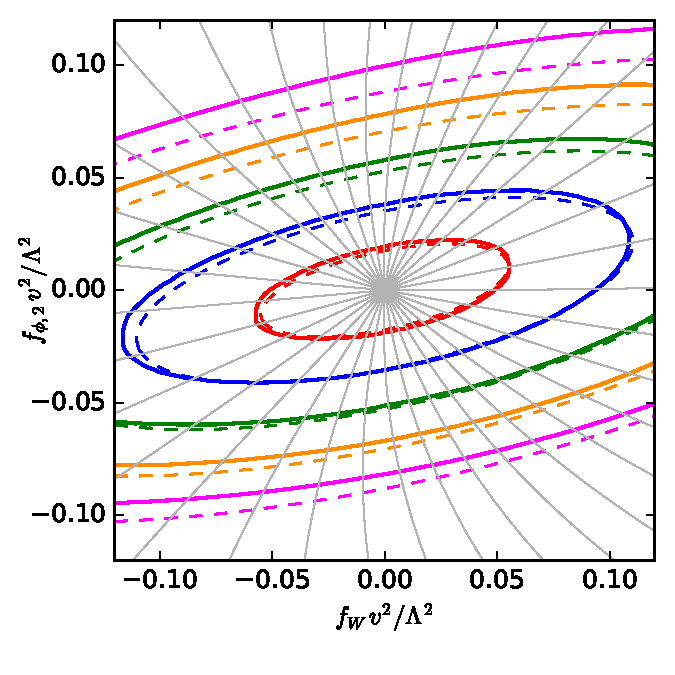
\includegraphics[height=0.33 \textwidth,clip,trim=0.3cm 0 0.05cm 0]{fig/information/wbf_tautau_geometry_fphi2_fw}%
  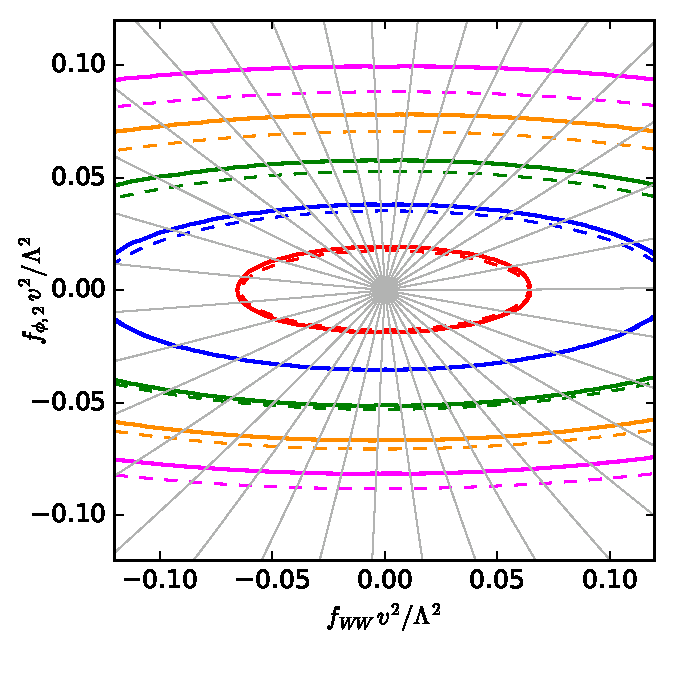
\includegraphics[height=0.33 \textwidth,clip,trim=0.3cm 0 0.05cm 0]{fig/information/wbf_tautau_geometry_fphi2_fww}%
  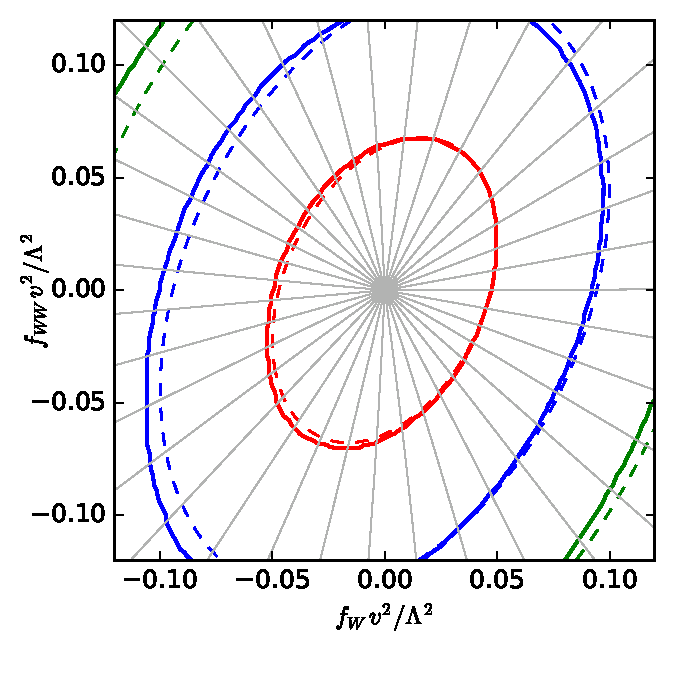
\includegraphics[height=0.33 \textwidth,clip,trim=0.3cm 0 0.05cm 0]{fig/information/wbf_tautau_geometry_fww_fw}%
  \caption{Error ellipses defined by the Fisher information in the WBF
    $H \to \tau \tau$ channel. We show contours of local distance
    $d_\text{local}(\boldtheta ; \boldzero)$ (dashed) and global distance
    $d(\boldtheta,\boldzero)$ (solid).  The colored contours indicate
    distances of $d = 1~...~5$. In grey we show example geodesics. The
    $\theta_i$ not shown are set to zero. }
\label{fig:information_wbf_tautau_geometry}
\end{figure}


Following \autoref{eq:def_wilson}, our model space is spanned by five
dimensionless parameters
%
\begin{align}
  \boldtheta = \frac {v^2} {\Lambda^2}  \fivevec {f_{\phi,2}} {f_W} {f_{WW}} {f_{B}}  {f_{BB}}  \,.
\label{eq:wilson_space_wbf}
\end{align}
%
With these basis vectors we calculate the Fisher information for
13~TeV using a combination of \toolfont{MadGraph5}~\cite{madgraph},
\toolfont{MadMax}~\cite{madmax2}, and our own \toolfont{MadFisher}
algorithm, described in Appendix~\ref{sec:information_algorithm}. We absorb the 
all particle identification and trigger efficiencies into a single universal $\varepsilon$
(which does not include the process-dependent CJV efficiencies). Then for our
toy example we assume the integrated luminosity times universal efficiencies to be 
$L \cdot \varepsilon  = 30~\ifb$. We find
%
\begin{align}
  I_{ij} (\mathbf{0}) =
\begin{pmatrix*}[r]
  3202.1 & -625.3 & -7.2 & -34.8 & 0.3 \\
  -625.3 & 451.0 & -109.5 & 23.3 & -1.5 \\
  -7.2 & -109.5 & 243.7 & -5.5 & 2.8 \\
  -34.8 & 23.3 & -5.5 & 4.1 & -0.3 \\
  0.3 & -1.5 & 2.8 & -0.3 & 0.1
\end{pmatrix*} \, .
\end{align}
%
The eigenvectors, ordered by the size of their eigenvalues, are
%
\begin{align}
  \boldtheta_1 = \fivevecr {0.98} {-0.21} {0.01} {-0.01} {0.00}  \qquad 
  \boldtheta_2 = \fivevecr {-0.18} {-0.79} {0.58} {-0.04} {0.01} \qquad 
  \boldtheta_3 = \fivevecr {0.12} {0.57} {0.81} {0.03} {0.01} \qquad 
  \boldtheta_4 = \fivevecr {0.00} {-0.05} {0.00} {1.00} {-0.07} \qquad 
  \boldtheta_5 = \fivevecr {0.00} {-0.00} {-0.01} {0.07} {1.00} \, .
\end{align}
%
The corresponding eigenvalues are $\left( 3338, 395, 165, 2.9, 0.1
\right)$, indicating that the WBF process has very different
sensitivities to the five operators: $\ope{\phi,2}$ can be most
strongly constrained and is weakly correlated with $\ope{W}$. It is
followed by the strongly correlated $\ope{W}$-$\ope{WW}$ plane.  The
sensitivity to $\ope{B}$ and $\ope{BB}$, which only play a role in
subleading $Z$-mediated production diagrams, is much smaller and shows
very little correlation with each other and everything else.

We visualize our results as contours of the local and global distances
defined in \autoref{eq:distances} for slices of parameter space in
\autoref{fig:information_wbf_tautau_geometry}.  First, the contours show the
maximum precision that can be attained in a measurement in this
process. Without taking into account systematic uncertainties, an
optimal measurement will probe the $\ope{\phi,2}$ direction with
$\Delta g \approx 0.02$, translating into
$\Lambda/\sqrt{f_{\phi,2}} \approx 1.8$~TeV. The $\ope{W}$ and
$\ope{WW}$ directions can optimally be probed at the
$\Delta g \approx 0.05$ or $\Lambda/\sqrt{f_{\phi,2}} \approx 1.1$~TeV
level.

Comparing the local and global distances provides some insight into
the role of $\ord{1/\Lambda^4}$ effects, as discussed before.  At $d =
1,2$ the differences are small, signaling that an optimal measurement
will be dominated by the linearized dimension-6 amplitudes. On the
other hand, analyses based on less luminosity or requiring more
stringent exclusion criteria (translating into larger distances) gain
sensitivity to the squared dimension-6 terms.



%%%%%%%%%%%%%%%%%%%%%%%%%%%%%%%%%%%%%%%%%%%%%%%%%%%%%%%%%%%%
\subsubsection*{Differential information}
%%%%%%%%%%%%%%%%%%%%%%%%%%%%%%%%%%%%%%%%%%%%%%%%%%%%%%%%%%%%

The fact that the Fisher information is additive across different
phase-space regions means that we can consider the differential
information with respect to phase space
($\diff I_{ij}/\diff\boldx$) or a specific kinematic
variable ($\diff I_{ij}/\diff\mathbf{v}$). In
\autoref{fig:information_wbf_tautau_differential_information} we show the
differential cross sections of the signal and dominant background
process for typical kinematic distributions and compare it to the
differential information.  More distributions are shown in
Appendix~\ref{sec:information_additional_plots}.

\begin{figure}
  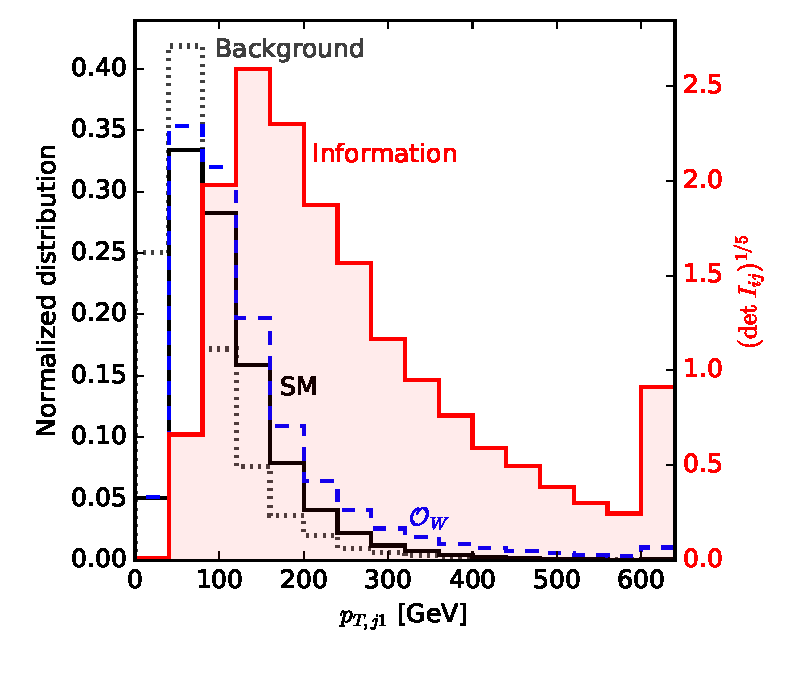
\includegraphics[height=0.45 \textwidth]{fig/information/wbf_tautau_information_over_ptj}%
  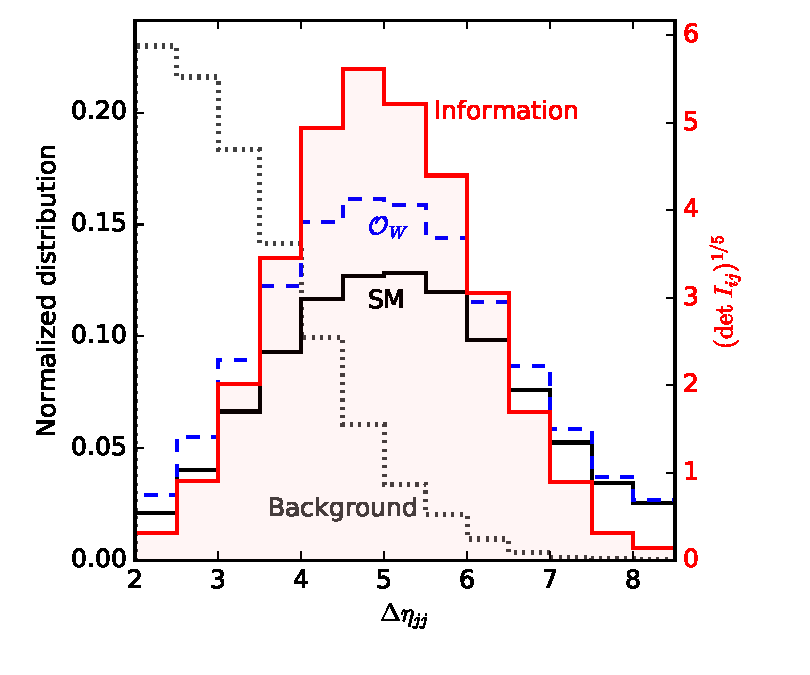
\includegraphics[height=0.45 \textwidth]{fig/information/wbf_tautau_information_over_deltaeta}%
  \caption{Distribution of the Fisher information in the WBF $H \to
    \tau \tau$ channel (shaded red). We also show the normalized SM signal
    (solid black) and QCD $Z$+jets (dotted grey) rates. The dashed blue line
    shows the effect of an exaggerated $f_{W} \, v^2 / \Lambda^2 =
    0.5$. The last bin is an overflow bin.}
  \label{fig:information_wbf_tautau_differential_information}
\end{figure}

Obviously, the signal-to-background ratio improves for large invariant
masses or the tagging jets and towards $m_{\tau \tau}$ values around
the Higgs mass. The information is larger in these phase-space
regions, independent of the direction in model space.  On the other
hand, most of our dimension-6 operators include derivatives, leading
to an increasing amplitude with momentum transfer through the
gauge-Higgs vertex. This momentum flow is not observable, but the
transverse momenta of the tagging jets and the Higgs boson are
strongly correlated with it~\cite{eft-edge}. Indeed most of the
information on higher-dimensional operators comes from the high-energy
tail of $p_{T,j_1}$.

The rapidity difference between the tagging jets indicates a trade-off
between these two effects: on the one hand, at larger rapidity
distances the signal-to-background ratio clearly
improves~\cite{phi_jj}. On the other hand, the largest effects from
dimension-6 operators appear at smaller $\Delta \eta_{jj}$, again
driven by the larger momentum transfer~\cite{eft-edge}. In the right panel of
\autoref{fig:information_wbf_tautau_differential_information} we see that the
information on these operators comes from $\Delta \eta_{jj} =
3\dots7$. Tight cuts with the aim to remove backgrounds lose a sizable
fraction of the information on dimension-6 operators.



%%%%%%%%%%%%%%%%%%%%%%%%%%%%%%%%%%%%%%%%%%%%%%%%%%%%%%%%%%%%
\subsubsection*{Information in distributions}
%%%%%%%%%%%%%%%%%%%%%%%%%%%%%%%%%%%%%%%%%%%%%%%%%%%%%%%%%%%%

\begin{figure}
  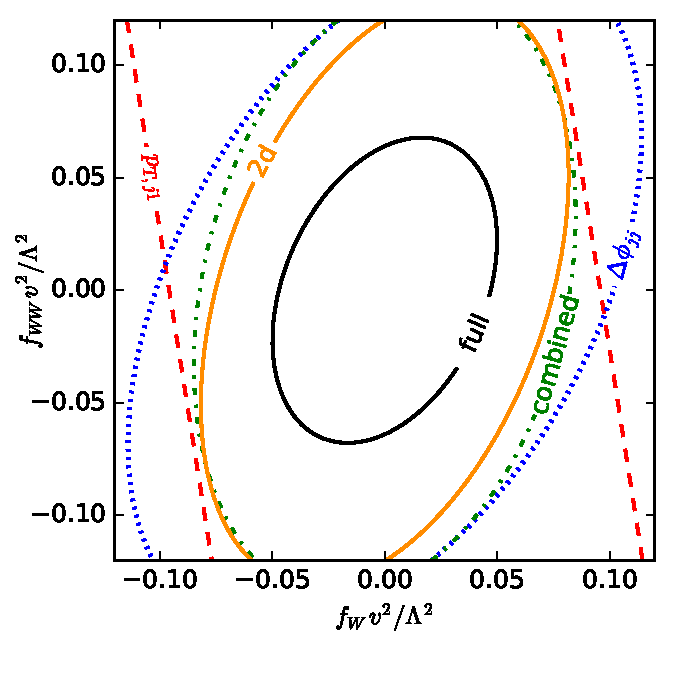
\includegraphics[height=0.45 \textwidth]{fig/information/wbf_tautau_histos_contours}
  \caption{Information from histograms compared to the full
    information  (black) in the WBF $H \to \tau \tau$ channel, shown as contours
    $d_{\text{local}}(\boldtheta ; \boldzero) = 1$. We include
    $p_{T,j_1}$, $\Delta \phi_{jj}$, their naive combination assuming
    no mutual information, and their two-dimensional histogram. The
    $\theta_i$ not shown are set to zero.}
  \label{fig:information_wbf_tautau_histograms_contours}
\end{figure}

While the integrated, fully differential information defined in
\autoref{eq:fisher_rates} provides us with optimal experimental
results, it remains to be shown that we can access it in
practice. Recent proposals using machine learning for high-dimensional
likelihood fits aim to tackle eactly this problem~\cite{machine_learning}.
Regardless, a relevant question is how much of this maximum
information is retained in simple one-dimensional or two-dimensional
distributions of standard kinematic observables $\mathbf{v}$. 

In the presence of backgrounds, a histogram-based analysis first
requires a stringent event selection. We choose the WBF cuts 
%
\begin{align}
  p_{T,j_1} > 50~\gev \qqqquad
  m_{jj} > 1~\tev \qqqquad
  \Delta \eta_{jj} > 3.6 \,.
  \label{eq:wbf_tautau_wbfcuts}
\end{align}
%
This improves the signal-to-background ratio to approximately unity,
but at the cost of losing discrimination power. Eventually, a
histogram-based analysis will benefit from optimizing this selection,
for instance foregoing the simple cuts for a multivariate approach,
going beyond the scope of this demonstration.  Based on this
selection, we analyze the distributions
%
\begin{itemize}
\item $p_{T,\tau_1}$ with bin size 25~GeV up to 500~GeV and an
  overflow bin;
\item $m_{\tau \tau}$ with bin size 5~GeV in the allowed range of
  $105~...~165~\gev$.
\item $p_{T,\tau \tau}$ with bin size 50~GeV up to 800~GeV and an
  overflow bin;
\item $p_{T,j_1}$ with bin size 50~GeV up to 800~GeV and an
  overflow bin;
\item $m_{jj}$ with bin size 250~GeV up to 4~TeV and an overflow
  bin;
\item $\Delta \eta_{jj}$ with bin size $0.5$ up to $8.0$ and an
  overflow bin;
\item $\Delta \phi_{jj} = \phi_{j_{\eta < 0}} - \phi_{j_{\eta > 0}}$~\cite{phi_jjs} with bin size $2 \pi / 20$;
\item $\Delta \eta_{\tau\tau, j1}$ with bin size $0.5$ up to $8.0$ and an
  overflow bin;
\item $\Delta \phi_{\tau \tau, j1}$ with bin size $\pi / 10$.
\end{itemize}  

\begin{figure}
  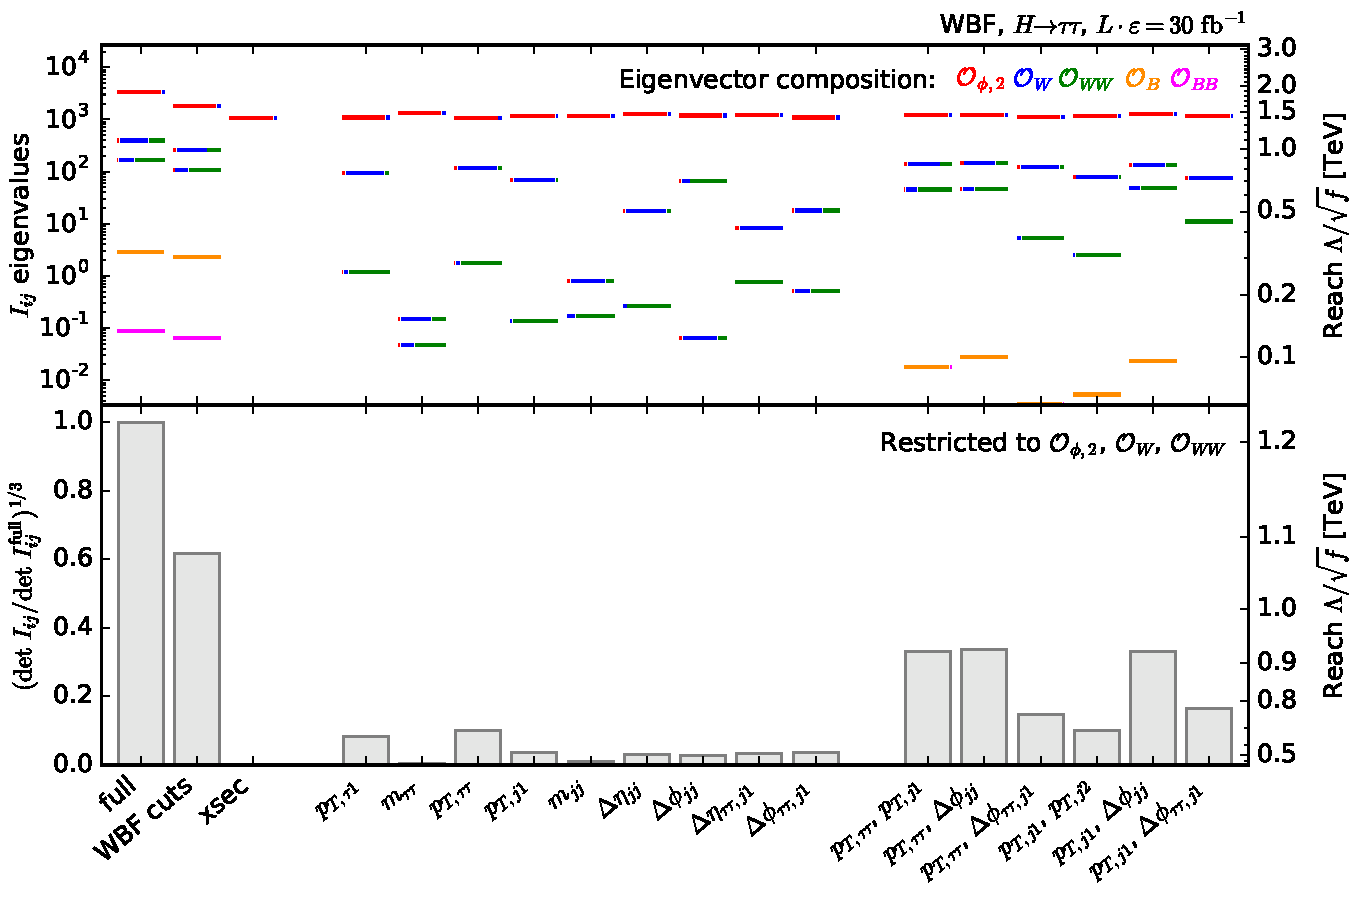
\includegraphics[height=0.6 \textwidth]{fig/information/wbf_tautau_histos_comparison}
  \caption{Fisher information for the WBF $H \to \tau \tau$ channel
    exploiting the full phase space, after the cuts in
    \autoref{eq:wbf_tautau_wbfcuts}, and for several kinematic
    distributions.  The top panel shows the eigenvalues, the colors
    denote the composition of the corresponding eigenvectors. The
    right axis translates the eigenvalues into a new physics reach for
    the corresponding combination of Wilson coefficients.  In the
    bottom panel we show the determinants of the Fisher information
    restricted to $\ope{\phi,2}$, $\ope{W}$, and $\ope{WW}$,
    normalized to the full information. Again, the right axis
    translates them into a new physics reach.}
\label{fig:information_wbf_tautau_histograms_comparison}
\end{figure}

\autoref{fig:information_wbf_tautau_histograms_contours} demonstrates that
virtuality measures such as the transverse momentum of the leading
tagging jet mostly constrain $\ope{W}$, while angular correlations
between the jets are more sensitive to $\ope{WW}$. Stringent
constraints on the full operator space can only be achieved by
combining the information in these distributions, ideally in a
two-dimensional histogram.

In \autoref{fig:information_wbf_tautau_histograms_comparison} we extend our
comparison to the information in all of the above distributions. The
top panel shows the eigenvalues of the individual information
matrices, and the colors indicate which operators the corresponding
eigenvectors are composed of. This allows us to see which operators
can be measured well in which distributions, and where blind (or flat)
directions arise. In the lower panel we compare the determinants,
providing a straightforward measure of the information in
distributions that is invariant under basis rotations. 

In general, single differential cross sections probe individual
directions in phase space well, but always suffer from basically blind
directions. To maximize the constraining power on all operators we
need to combine virtuality measures and angular correlations. Even
then there is a substantial difference to the maximum information in
the process: the combined analysis of jet transverse momenta and
$\Delta \phi_{jj}$ has a new physics reach in the
$\ope{\phi,2}$-$\ope{W}$-$\ope{WW}$ space of $0.9~\tev$, compared to
$1.2~\tev$ for the fully differential cross section.  Under our
simplistic assumptions this corresponds to roughly three times more
data.  Half of this loss in constraining power is due to information
in background-rich regions discarded by the WBF cuts, and half is due
to non-trivial kinematics not captured by the double differential
distributions.



%%%%%%%%%%%%%%%%%%%%%%%%%%%%%%%%%%%%%%%%%%%%%%%%%%%%%%%%%%%%
\subsection{Weak-boson-fusion Higgs to four leptons}
\label{sec:information_wbf_4l}
%%%%%%%%%%%%%%%%%%%%%%%%%%%%%%%%%%%%%%%%%%%%%%%%%%%%%%%%%%%%

Another question we can approach with information geometry is how much
the non-trivial decay mode $H \to 4 \ell$ adds to the WBF production
analyzed in \autoref{sec:information_wbf_taus}. For this particularly clean
channel, shown in \autoref{fig:information_wbf_4l_diag}, the backgrounds are
not the limiting factor, so we omit them for our toy study. This also 
allows us to avoid smearing the $m_{4\ell}$ distribution. At parton
level we apply the generator-level cuts
%
\begin{alignat}{2}
  p_{T,j} &> 20 \ \gev \qquad & \qquad |\eta_{j}| &< 5.0  \notag \\ 
  p_{T,\ell} &> 10 \ \gev  \qquad & \qquad |\eta_{\ell}| &< 2.5 \; ,
\label{eq:wbf_4l_acceptance_cuts}
\end{alignat}
%
with $\ell = e, \mu$. The SM cross section after these cuts is 0.36~fb.



%%%%%%%%%%%%%%%%%%%%%%%%%%%%%%%%%%%%%%%%%%%%%%%%%%%%%%%%%%%%
\subsubsection*{Maximum precision on Wilson coefficients}
%%%%%%%%%%%%%%%%%%%%%%%%%%%%%%%%%%%%%%%%%%%%%%%%%%%%%%%%%%%%

Again we study the five-dimensional space of CP-even Wilson
coefficients given in \autoref{eq:wilson_space_wbf}.  For increased
luminosity, $L \cdot \varepsilon = 100~\ifb$, we find the SM
information
%
\begin{align}
  I_{ij} (\boldzero) =
\begin{pmatrix*}[r]
  144.3 & -27.3 & -11.5 & -1.6 & -0.7 \\
  -27.3 & 50.9 & -9.1 & 6.7 & -0.2 \\
  -11.5 & -9.1 & 36.9 & -1.2 & 1.0 \\
  -1.6 & 6.7 & -1.2 & 1.9 & -0.1 \\
  -0.7 & -0.2 & 1.0 & -0.1 & 0.1
\end{pmatrix*}
\end{align}
%
with the eigenvectors 
%
\begin{align}
  \boldtheta_1 = \fivevecr {0.96} {-0.25} {-0.08} {-0.02} {0.00}  \qquad 
  \boldtheta_2 = \fivevecr {-0.16} {-0.79} {0.58} {-0.11} {0.02}  \qquad
  \boldtheta_3 = \fivevecr {0.21} {0.54} {0.81} {0.09} {0.02} \qquad 
  \boldtheta_4 = \fivevecr {0.02} {0.14} {0.01} {-0.99} {0.04}  \qquad 
  \boldtheta_5 = \fivevecr {0.00} {-0.00} {-0.03} {0.04} {1.00}  \,.
\end{align}
%
and the eigenvalues $\left( 152.4, 52.8, 27.8, 1.0, 0.0 \right)$. 

When we compare the above outcome to our earlier WBF production analysis we see
that the decay $H \to 4\ell$ does not increase the sensitivity to
$\ope{B}$ or $\ope{BB}$; both of them are still basically blind
directions. We visualize the information geometry in the remaining
directions in \autoref{fig:information_wbf_4l_geometry}. The differences between
local and global distances are much larger than in the $H \to \tau
\tau$ channel. This is because the tiny $H \to 4\ell$ branching
fraction decreases the new physics reach and with it the hierarchy of
scales in our effective Lagrangian. This means that the squared
dimension-6 amplitudes are numerically more relevant.

\begin{figure}
  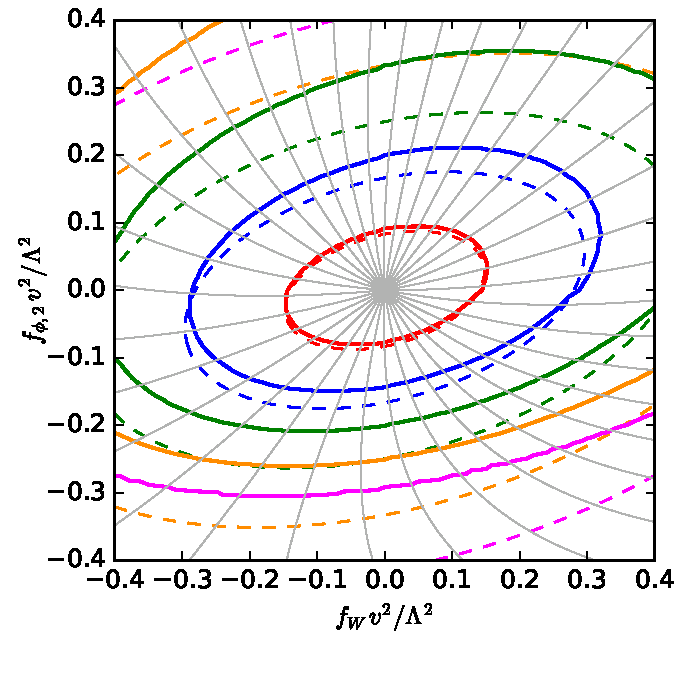
\includegraphics[height=0.33 \textwidth,clip,trim=0.3cm 0 0.05cm 0]{fig/information/wbf_4l_geometry_fphi2_fw}%
  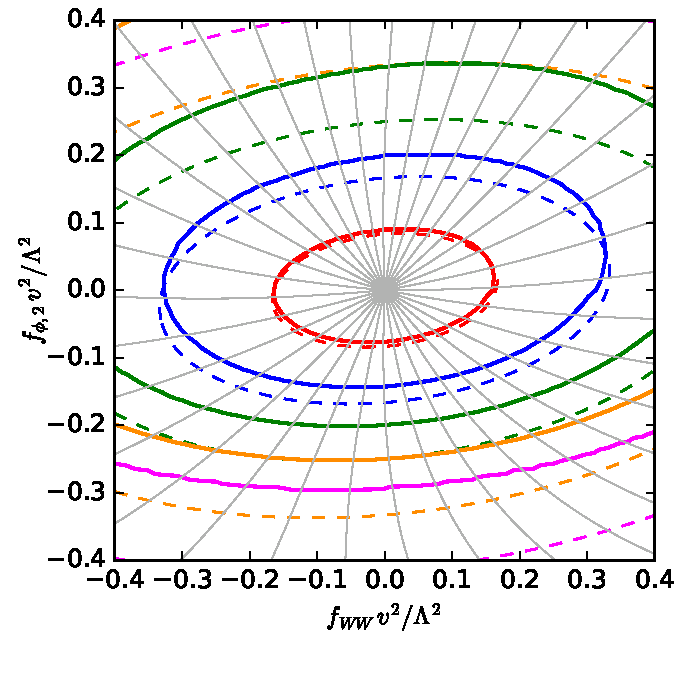
\includegraphics[height=0.33 \textwidth,clip,trim=0.3cm 0 0.05cm 0]{fig/information/wbf_4l_geometry_fphi2_fww}%
  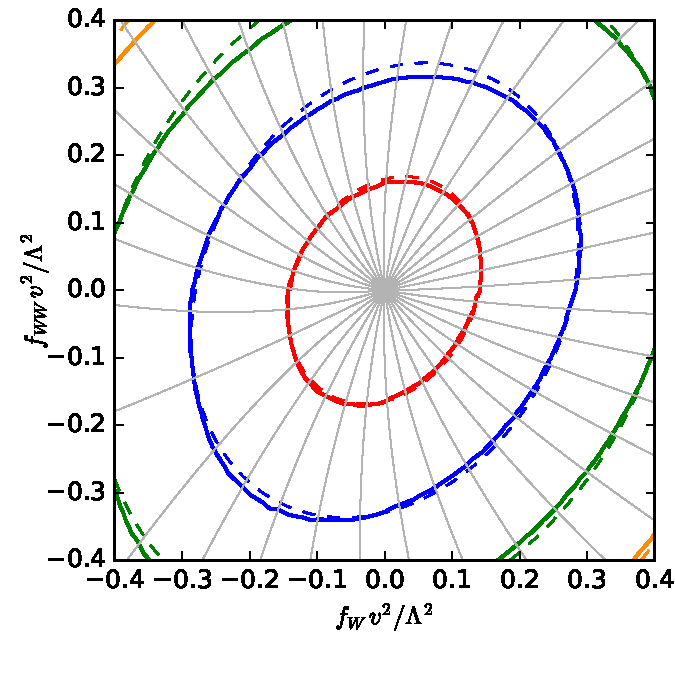
\includegraphics[height=0.33 \textwidth,clip,trim=0.3cm 0 0.05cm 0]{fig/information/wbf_4l_geometry_fww_fw}%
  \caption{Error ellipses defined by the Fisher information in the
    WBF $H \to 4\ell$ channel. We show contours of local distance
    $d_\text{local}(\boldtheta ; \boldzero)$ (dashed) and global
    distance $d(\boldtheta,\boldzero)$ (solid). The colored contours
    indicate distances of $d = 1~...~5$. In grey we show example
    geodesics.  The $\theta_i$ not shown are set to zero.}
\label{fig:information_wbf_4l_geometry}
\end{figure}



%%%%%%%%%%%%%%%%%%%%%%%%%%%%%%%%%%%%%%%%%%%%%%%%%%%%%%%%%%%%
\subsubsection*{Production vs decay kinematics}
%%%%%%%%%%%%%%%%%%%%%%%%%%%%%%%%%%%%%%%%%%%%%%%%%%%%%%%%%%%%

\begin{figure}
  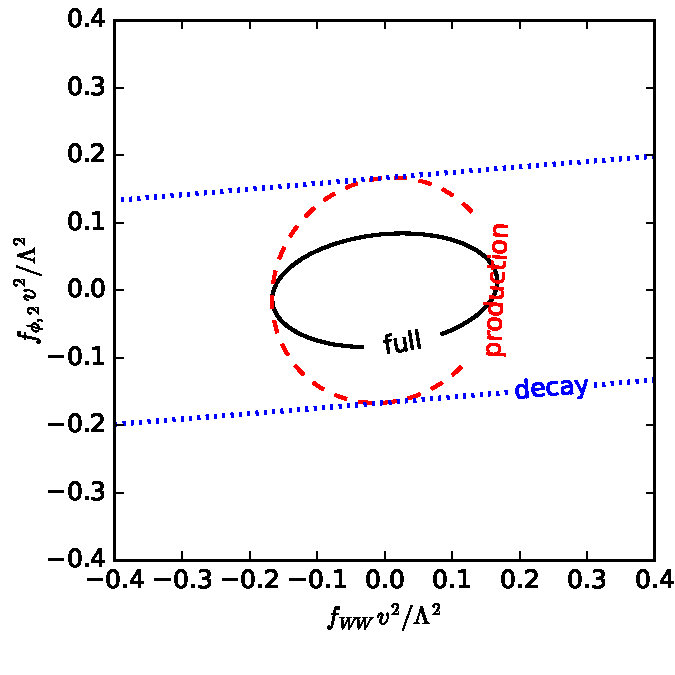
\includegraphics[height=0.45 \textwidth]{fig/information/wbf_4l_production_decay_fphi2_fww}
  \caption{Information in the WBF $H \to 4\ell$ channel from including
    dimension-6 operators only in the production vertex (red), only in
    the decay vertex (blue), and both (black). The information is
    visualized as local contours
    $d_{\text{local}}(\boldtheta ; \boldzero) = 1$. The $\theta_i$ not shown
    are set to zero.}
\label{fig:information_wbf_4l_production_decay}
\end{figure}

Focusing on the question how the decay analysis improves our global
information, we disentangle the effects on the production and decay
vertices in \autoref{fig:information_wbf_4l_production_decay}.  As well known for
the LHC, the production-side analysis benefits from a large momentum
flow through the Higgs vertex, while the momentum flow through the
decay vertices is bounded by the Higgs mass (neglecting off-shell
phase space regions).  For momentum-dependent operators this
disadvantage is not compensated by the complex $H \to 4\ell$ decay
kinematics.  Consequently, the Higgs decay only improves the reach in
the $\ope{\phi,2}$ direction, corresponding to a change in the total rate. 
This operator also affects many other total Higgs rates,
so we conclude that the complex $H \to 4\ell$ kinematics
does not play a significant role as part of a global analysis. 

\begin{figure}
  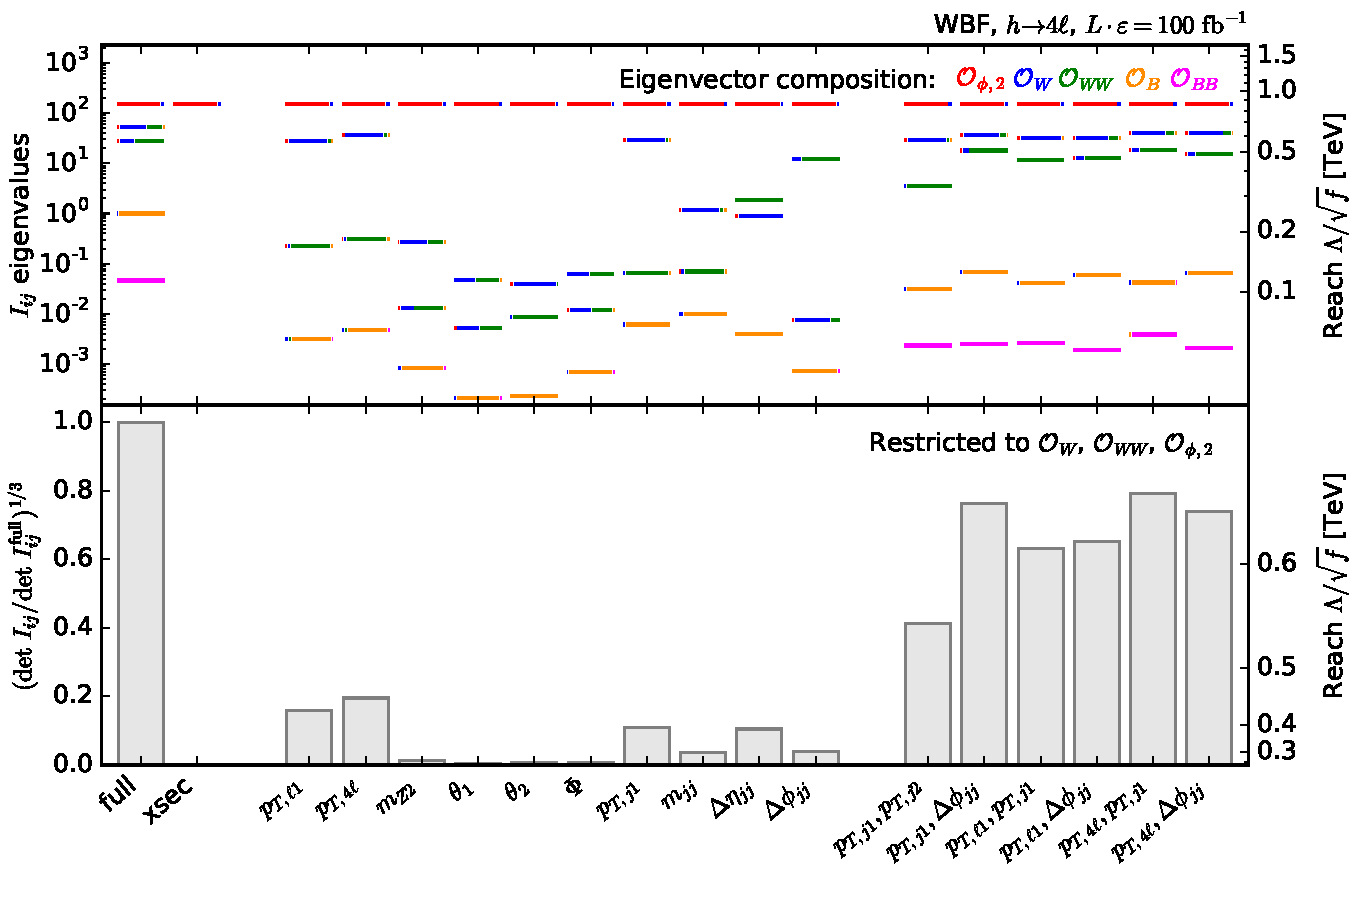
\includegraphics[height=0.6 \textwidth]{fig/information/wbf_4l_histos_comparison}
  \caption{Fisher information for the WBF $H \to 4 \ell$ channel
    exploiting the full phase space, after the cuts in
    \autoref{eq:wbf_tautau_wbfcuts}, and for several kinematic
    distributions.  The top panel shows the eigenvalues, the colors
    denote the composition of the corresponding eigenvectors. The
    right axis translates the eigenvalues into a new physics reach for
    the corresponding combination of Wilson coefficients.  In the
    bottom panel we show the determinants of the Fisher information
    restricted to $\ope{\phi,2}$, $\ope{W}$, and $\ope{WW}$,
    normalized to the full information. Again, the right axis
    translates them into a new physics reach.}
\label{fig:information_wbf_4l_histograms_comparison}
\end{figure}

In complete analogy to \autoref{fig:information_wbf_tautau_histograms_comparison}
for the WBF production, we compare the information in different
distributions for $CP$-even operators in
\autoref{fig:information_wbf_4l_histograms_comparison}.  The standard tagging jet
observables are complemented by five observables characterizing the
$4\ell$ decay kinematics,
%
\begin{itemize}
  \item $p_{T,\ell_1}$;
  \item $p_{T,4\ell}$;
  \item $m_{Z_2}$ for the lower-mass reconstructed $Z$ boson;
  \item $\cos \theta_1 = \hat{p}_{\ell^-_1} \cdot \hat{p}_{Z_2}
    \Big|_{Z_1}$ defined in terms of unit-3-vectors $\hat{p}$, and analogously
    $\cos \theta_2^*$;
  \item $\cos \Phi = ( \hat{p}_{\ell^-_1} \times
    \hat{p}_{\ell^+_1} ) \cdot ( \hat{p}_{\ell^-_2} \times
    \hat{p}_{\ell^+_2} )$, defined in the $ZZ$ or Higgs rest
    frame~\cite{phi_jj}.
\end{itemize}
%
In all cases we use at least ten bins and include underflow and
overflow bins where applicable.

In our quantitative analysis we find similar patterns as in the
$\tau \tau$ mode. The key observables are again transverse momenta and
jet angular correlations. Without the complication of removing
backgrounds efficiently, the combined analysis of these variables
comes close to the maximum information: a two-dimensional histogram of
jet transverse momenta and $\Delta \phi_{jj}$ probes new physics
scales up to 650~GeV, while for a fully differential analysis the
maximum probed new physics scale is close to 700~GeV. Under our
assumptions, this difference roughly corresponds to 25\% more
data. The decay kinematics and its angular observables do not help
significantly or change the picture qualitatively.  This shows again
how much the sensitivity of the decay vertices to dimension-6
operators is limited by the restriction of the momentum flow to the
Higgs mass. This is not accidental: the reason behind this role of the
momentum dependence is that for all operators shown in
\autoref{eq:wilson_space_wbf} with the exception of $\ope{\phi,2}$,
gauge invariance forces us to include the field strength tensor
instead of the gauge boson field, automatically introducing a momentum
dependence.



%%%%%%%%%%%%%%%%%%%%%%%%%%%%%%%%%%%%%%%%%%%%%%%%%%%%%%%%%%%%
\subsection{Higgs plus single top}
\label{sec:information_th}
%%%%%%%%%%%%%%%%%%%%%%%%%%%%%%%%%%%%%%%%%%%%%%%%%%%%%%%%%%%%

Our final example is Higgs production with a single top with
$H\to \gamma \gamma$ and a hadronic top decay. As shown in
\autoref{fig:information_th_diag}, diagrams where the Higgs is
radiated off a $W$ boson interfere destructively with diagrams with a
top-Higgs coupling, making this channel a direct probe of the sign of
the top Yukawa coupling~\cite{top_higgs}. We stick to a parton-level
analysis at leading order in the five-flavor scheme. For our toy
example we include only one of the dominant backgrounds, single top
production with two photons, and in particular ignore the multi-jet
background. The subleading $t\bar{t} \, \gamma\gamma$ background
populates qualitatively different phase-space regions from the
single-top signal and can be supressed with an appropriate event
selection~\cite{Kling:2012up}. We smear the $m_{\gamma \gamma}$
distribution of the signal process with a Gaussian of width 1.52 GeV
estimated from Figure~6b of Reference~\cite{CMS:2016zjv}, and do not
include any other detector effects. Our basic event selection requires
%
\begin{alignat}{4}
  p_{T,j} &> 20 \ \gev \quad & \quad
  |\eta_{j}| &< 5.0 \quad & \quad
  \Delta R_{jj} &> 0.4 \quad & \quad
  152 \ \gev &<m_{bjj} < 192 \ \gev \notag \\ 
  p_{T,\gamma} &> 10 \ \gev \quad & \quad
  |\eta_{\gamma}| &< 2.5 \quad & \quad 
  \Delta R_{\gamma j} , \Delta R_{\gamma \gamma} &> 0.4 \quad & \quad
  120 \ \gev &<m_{\gamma \gamma} < 130 \ \gev \,,
  \label{eq:th_acceptance_cuts}
\end{alignat}
%
leading to a SM $tH$ cross section of 0.10~fb and a background of 0.22~fb.

We consider four $CP$-even dimension-6 operators
%
\begin{alignat}{2}
  \ope{W}  &= i \frac{g}{2} \, (D^\mu\phi)^\dagger \sigma^k ( D^\nu\phi) \, W_{\mu\nu}^k  \qquad & \qquad
  \ope{t \phi}  &= (\phisq) \, ( \overbar{Q}_3 \tilde{\phi} t_R)  + \text{h.c.} \notag \\
  \ope{WW}  &= -\frac{g^2}{4} \, (\phisq) \, W^k_{\mu\nu} \, W^{\mu\nu\, k}  \qquad & \qquad
  \ope{\phi,2}  &= \frac{1}{2} \, \partial^\mu(\phi^\dagger\phi) \, \partial_\mu(\phi^\dagger\phi) \,.
\label{eq:th_ope}
\end{alignat}
%
The operators $\ope{W}$ and $\ope{WW}$ affect the production amplitudes where
the Higgs couples to a $W$, while $\ope{t \phi}$ re-scales the top
Yukawa coupling. Both, $\ope{WW}$ and $\ope{\phi,2}$ also affect the
$H \to \gamma \gamma$ decay.


%%%%%%%%%%%%%%%%%%%%%%%%%%%%%%%%%%%%%%%%%%%%%%%%%%%%%%%%%%%%
\subsubsection*{Maximum precision on Wilson coefficients}
%%%%%%%%%%%%%%%%%%%%%%%%%%%%%%%%%%%%%%%%%%%%%%%%%%%%%%%%%%%%

\begin{figure}
  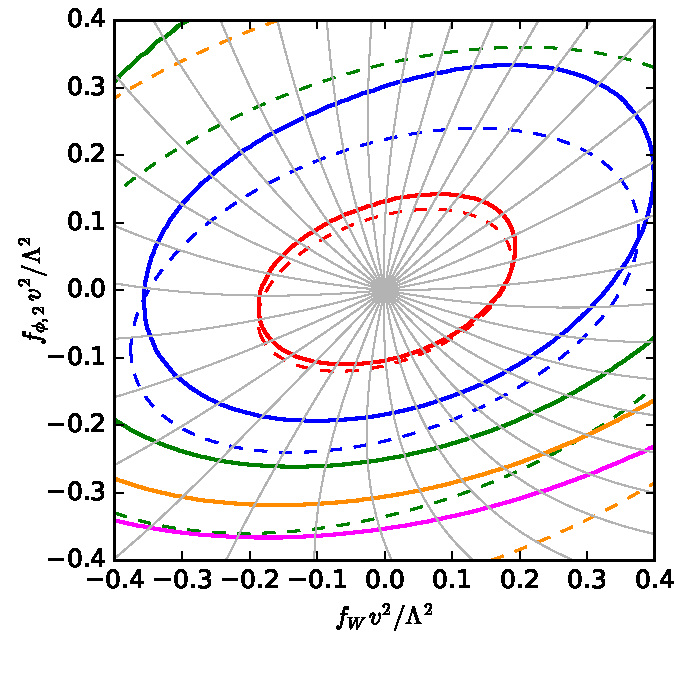
\includegraphics[height=0.33 \textwidth,clip,trim=0.3cm 0 0.05cm 0]{fig/information/th_geometry_fphi2_fw}%
  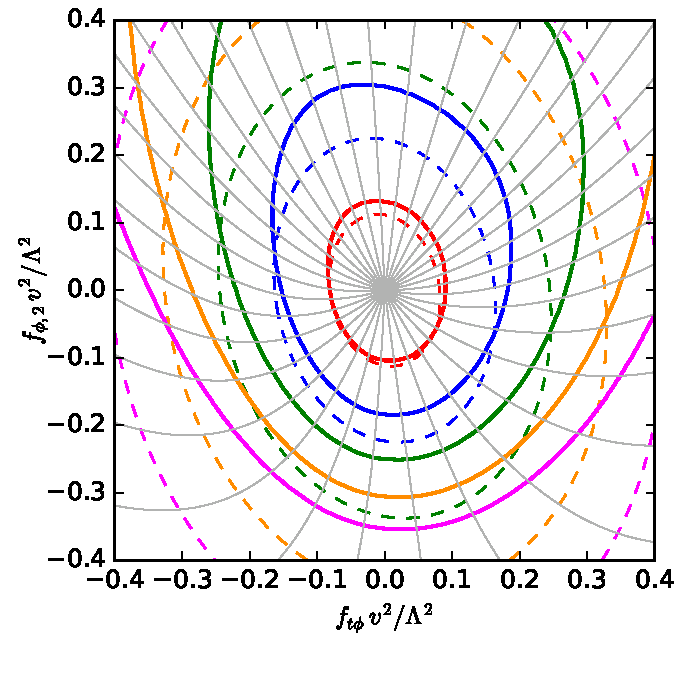
\includegraphics[height=0.33 \textwidth,clip,trim=0.3cm 0 0.05cm 0]{fig/information/th_geometry_fphi2_ftphi}%
  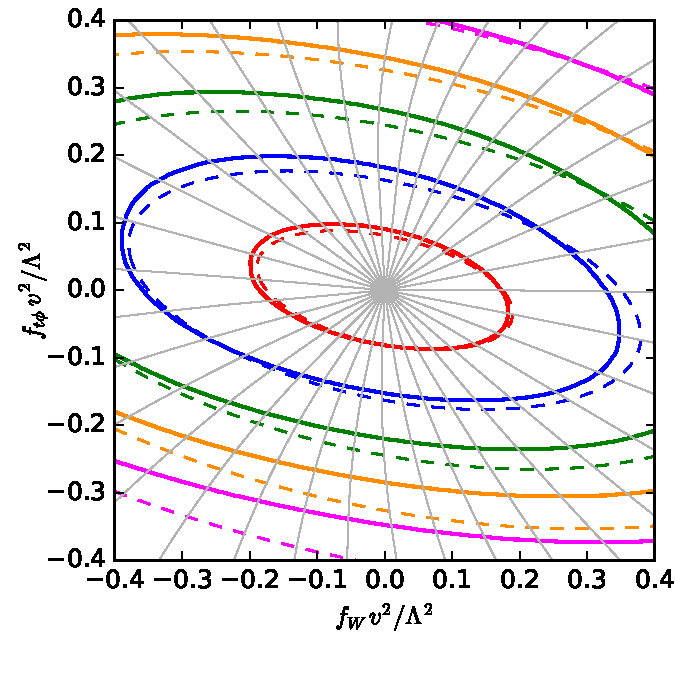
\includegraphics[height=0.33 \textwidth,clip,trim=0.3cm 0 0.05cm 0]{fig/information/th_geometry_ftphi_fw}%
  \caption{Error ellipses defined by the Fisher information in Higgs
    plus single top production. We show contours of local distance
    $d_\text{local}(\boldtheta ; \boldzero)$ (dashed) and global distance
    $d(\boldtheta,\boldzero)$ (solid).  The colored contours indicate
    distances of $d = 1~...~5$. In grey we show example geodesics. The
    $\theta_i$ not shown are set to zero. }
\label{fig:information_th_geometry}
\end{figure}


We calculate the Fisher information in terms of the dimensionless parameters
%
\begin{align}
  \boldtheta = \frac {v^2} {\Lambda^2}  \fourvec {f_{\phi,2}} {f_W} {f_{WW}} {f_{t \phi}}
  \label{eq:wilson_space_th}
\end{align}
%
for 13~TeV and an integrated luminosity times efficiencies of
$L \cdot \varepsilon = 300~\ifb$ and find
%
\begin{align}
  I_{ij} (\mathbf{0}) =
\begin{pmatrix*}[r]
  80.1 & -18.7 & -957.0 & 13.2 \\
  -18.7 & 32.6 & 221.7 & 27.0 \\
  -957.0 & 221.7 & 11446.1 & -146.0 \\
  13.2 & 27.0 & -146.0 & 150.3
\end{pmatrix*} \, .
\end{align}
%
The eigenvectors are
%
\begin{align}
  \boldtheta_1 = \fourvecr {0.08} {-0.02} {-1.00} {0.01}  \qquad 
  \boldtheta_2 = \fourvecr {0.00} {-0.23} {-0.01} {-0.97} \qquad 
  \boldtheta_3 = \fourvecr {-0.02} {0.97} {-0.02} {-0.23} \qquad 
  \boldtheta_4 = \fourvecr {1.00} {0.02} {0.08} {-0.01}
\end{align}
%
with corresponding eigenvalues $\left( 11532, 155, 21.3, 0.1 \right)$.
The best constrained direction along $\ope{WW}$ corresponds to the
combination of Wilson coefficients that affects the
$H \to \gamma \gamma$ decay in addition to production effects, which
will already be tightly constrained once a $tH$ measurement is
feasible. The orthogonal direction in the $\ope{\phi,2}$-$\ope{W}$
plane is for all practical purposes blind. Even with the assumed
sizeable event rate corresponding to 300~$\ifb$, the sensitivity to
$\ope{W}$ and $\ope{t \phi}$ is limited, with some mixing between the
two operators.

We visualize this maximum sensitivity to dimension-6 operators in
\autoref{fig:information_th_geometry}. With the exception of $\ope{WW}$, an
optimal measurement can probe all operators at the
$\Delta g \approx 0.1\dots 0.2$ level, equivalent to
$\Lambda/\sqrt{f_{\phi,2}} \approx 600 \dots 750$~GeV.  There are
large differences between local and global distances already at the
$d = 2$ level, implying that a measurement of this channel will always
be sensitive to the squared dimension-6 terms.



%%%%%%%%%%%%%%%%%%%%%%%%%%%%%%%%%%%%%%%%%%%%%%%%%%%%%%%%%%%%
\subsubsection*{Differential information}
%%%%%%%%%%%%%%%%%%%%%%%%%%%%%%%%%%%%%%%%%%%%%%%%%%%%%%%%%%%%

\begin{figure}
  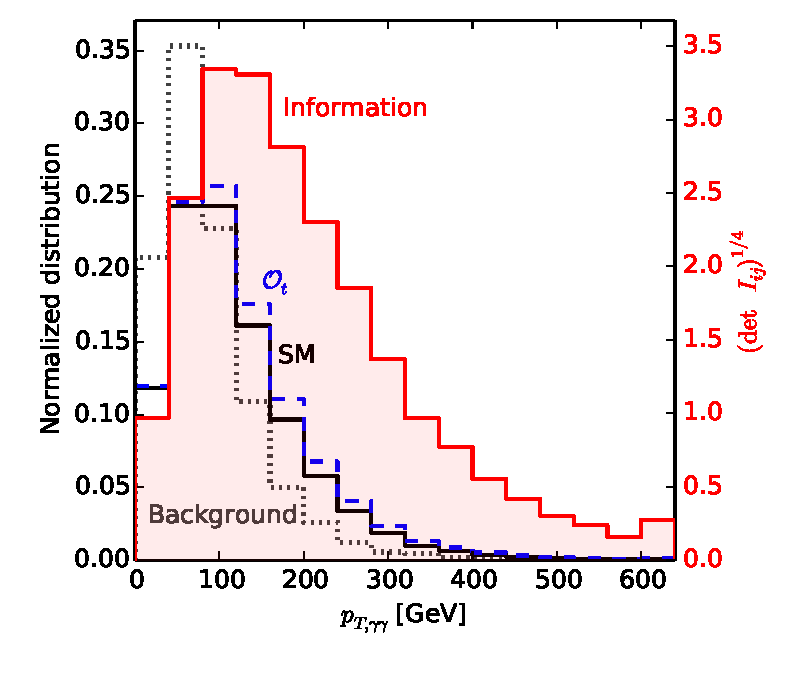
\includegraphics[height=0.45 \textwidth]{fig/information/th_information_over_ptaa}%
  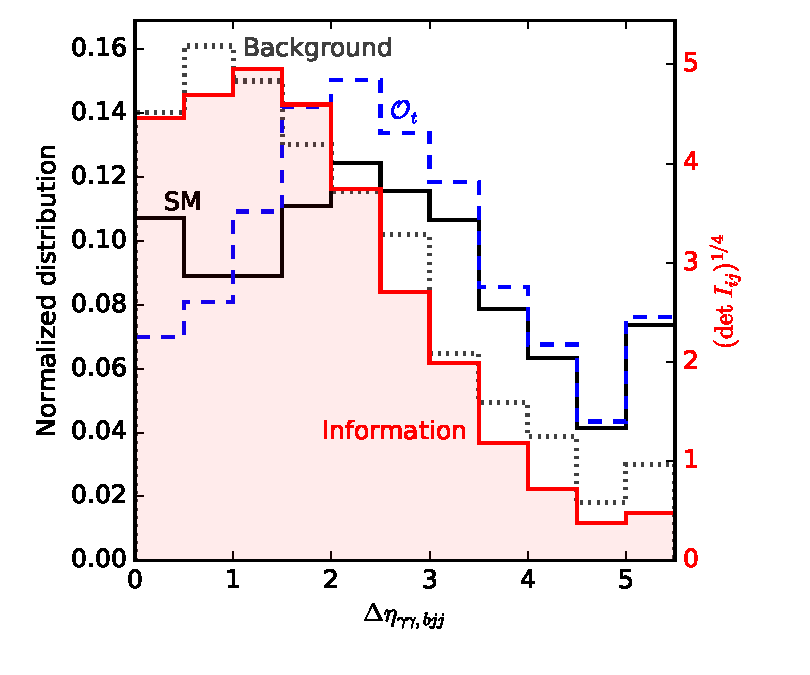
\includegraphics[height=0.45 \textwidth]{fig/information/th_information_over_deltaeta}%
  \caption{Distribution of the Fisher information in the Higgs plus
    single top channel (shaded red). We also show the normalized SM
    signal (solid black) and single-top background (dotted grey)
    rates. The dashed blue line shows the effect of
    $f_{t \phi} \, v^2 / \Lambda^2 = 0.2$. The last bin is an overflow
    bin.}
  \label{fig:information_th_differential_information}
\end{figure}

In \autoref{fig:information_th_differential_information} we show the distribution
of this information over phase space. More distributions are shown in
Appendix~\ref{sec:information_additional_plots}. As expected, the information is
concentrated in the $m_{\gamma \gamma} \sim m_H$ peak and in the
high-energy tails of transverse momenta. Studying angular correlations
between the Higgs system and the top decay products, we find that the
region $\Delta \eta_{ \gamma \gamma, bjj} \lesssim 3$ contains a lot
of discrimination power.




%%%%%%%%%%%%%%%%%%%%%%%%%%%%%%%%%%%%%%%%%%%%%%%%%%%%%%%%%%%%
\subsubsection*{Information in distributions}
%%%%%%%%%%%%%%%%%%%%%%%%%%%%%%%%%%%%%%%%%%%%%%%%%%%%%%%%%%%%

In a next step, we compare this full information to the reduced
information in one-dimensional and two-dimensional distributions of
kinematic observables. We now require harder cuts
%
\begin{align}
  p_{T,j_1} > 50~\gev \qquad 
  p_{T,\gamma} > 50,~30~\gev \qquad
  122~\gev < m_{\gamma \gamma} < 128~\gev \,,
  \label{eq:th_cuts}
\end{align}
%
which reduces the background to the level of the signal. We then
analyze the distributions~\cite{top_higgs,Kling:2012up}
%
\begin{itemize}
\item $p_{T,\gamma_1}$ with bin size 25~GeV up to 400~GeV and an
  overflow bin;
\item $m_{\gamma\gamma}$ with bin size 1~GeV in the allowed range of
  $123~...~127~\gev$;
\item $p_{T,\gamma \gamma}$ with bin size 40~GeV up to 600~GeV and an
  overflow bin;
\item $\Delta \phi_{\gamma \gamma}$ with bin size $\pi/10$;  
\item $p_{T,j_1}$ with bin size 40~GeV up to 400~GeV and an
  overflow bin;
\item $p_{T,b}$ with bin size 40~GeV up to 400~GeV and an
  overflow bin;
\item $p_{T,bjj}$ with bin size 40~GeV up to 600~GeV and an
  overflow bin;
\item $\Delta \phi_{\gamma \gamma, b}$ with bin size $\pi / 10$;
\item $\Delta \eta_{\gamma\gamma, b}$ with bin size $0.5$ up to $5.0$ and an
  overflow bin;
\item $m_{\gamma \gamma bjj}$ with bin size 100~GeV up to 1500~GeV and an
  overflow bin;
\item $p_{T,\gamma \gamma bjj}$ with bin size 40~GeV up to 400~GeV and an
  overflow bin;
\item $\Delta \phi_{\gamma \gamma, bjj}$ with bin size $\pi / 10$;
\item $\Delta \eta_{\gamma\gamma, bjj}$ with bin size $0.5$ up to $5.0$ and an
  overflow bin.
\end{itemize} 

\begin{figure}
  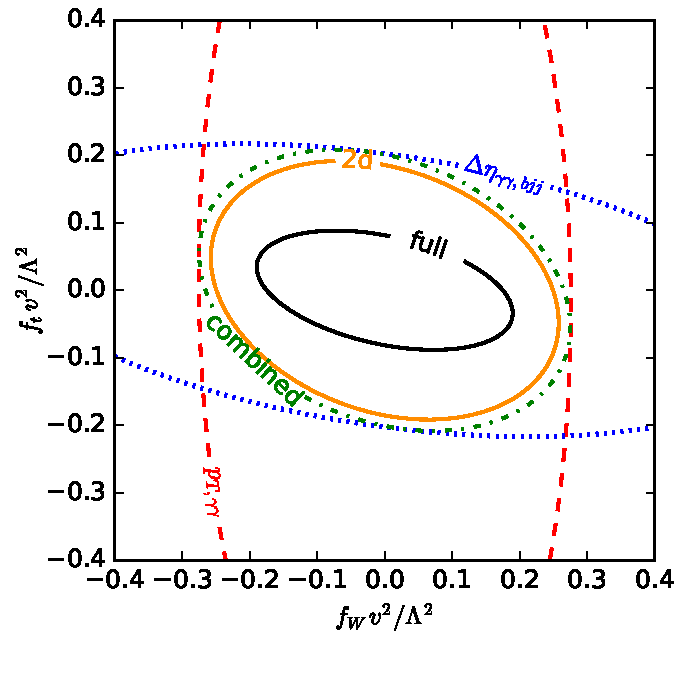
\includegraphics[height=0.45 \textwidth]{fig/information/th_histos_contours}
  \caption{Information from histograms compared to the full
    information (black), shown as contours
    $d_{\text{local}}(\boldtheta ; \boldzero) = 1$. We include
    $p_{T,\gamma \gamma}$, $\Delta \eta_{\gamma\gamma, bjj}$, their naive combination assuming
    no mutual information, and their two-dimensional histogram. The
    $\theta_i$ not shown are set to zero.}
  \label{fig:information_th_histograms_contours}
\end{figure}

As in the WBF case, different observables probe different Wilson
operators. \autoref{fig:information_wbf_tautau_histograms_contours} shows that
the di-photon transverse momentum constrains mostly the $\ope{W}$
direction, while the rapidity separation between the Higgs and top
systems is more sensitive to $\ope{t\phi}$.

\begin{figure}
  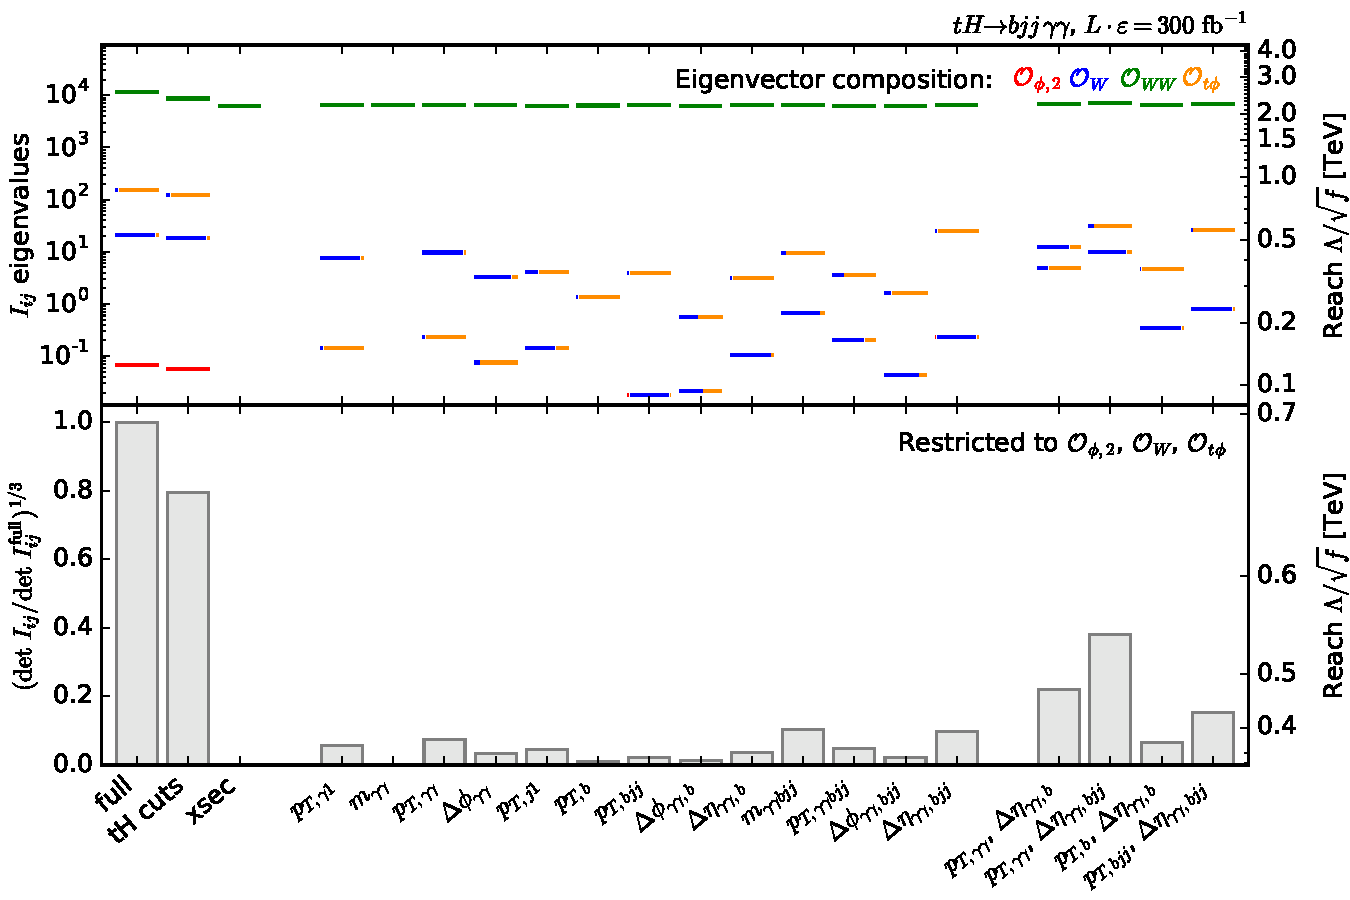
\includegraphics[height=0.6 \textwidth]{fig/information/th_histos_comparison}
  \caption{Fisher information for the Higgs plus single top channel
    exploiting the full phase space, after the cuts in
    \autoref{eq:th_cuts}, and for several kinematic distributions.
    The top panel shows the eigenvalues, the colors denote the
    composition of the corresponding eigenvectors. The right axis
    translates the eigenvalues into a new physics reach for the
    corresponding combination of Wilson coefficients.  In the bottom
    panel we show the determinants of the Fisher information
    restricted to $\ope{\phi,2}$, $\ope{W}$, and $\ope{t\phi}$,
    normalized to the full information. Again, the right axis
    translates them into a new physics reach.}
\label{fig:information_th_histograms_comparison}
\end{figure}

In \autoref{fig:information_th_histograms_comparison} we compare the eigenvalues,
eigenvectors and determinants of the information matrices in all of
the above distributions. We confirm that the photon observables mostly
probe changes in the Higgs-gauge coupling from $\ope{W}$, while a
rescaled top Yukawa will be visible in the properties of the top decay
products. Distributions of the properties of the $b$ jet consistently
contain significantly less information than the corresponding
distributions for the reconstructed top system. The rapidity
difference between the $\gamma \gamma$ system and the reconstructed
top provides a particularly good probe of this
operator~\cite{top_higgs}. Combining this variable with the transverse
momentum of the $\gamma \gamma$ system we can probe new physics scales
in the $\ope{W}$-$\ope{t\phi}$ plane around 550~GeV in the
$\ope{W}$-$\ope{WW}$-$\ope{\phi,2}$ space, compared to 700~GeV for the
fully differential cross section. This corresponds to almost three
times more data under our simplifying assumptions.



%%%%%%%%%%%%%%%%%%%%%%%%%%%%%%%%%%%%%%%%%%%%%%%%%%%%%%%%%%%%
\section{$CP$ violation in the Higgs sector}
\label{sec:information_application_odd}
%%%%%%%%%%%%%%%%%%%%%%%%%%%%%%%%%%%%%%%%%%%%%%%%%%%%%%%%%%%%




%%%%%%%%%%%%%%%%%%%%%%%%%%%%%%%%%%%%%%%%%%%%%%%%%%%%%%%%%%%%
\section{Technical questions}
\label{sec:information_extensions}
%%%%%%%%%%%%%%%%%%%%%%%%%%%%%%%%%%%%%%%%%%%%%%%%%%%%%%%%%%%%

%%%%%%%%%%%%%%%%%%%%%%%%%%%%%%%%%%%%%%%%%%%%%%%%%%%%%%%%%%%%
\subsection{Systematic uncertainties}
 %%%%%%%%%%%%%%%%%%%%%%%%%%%%%%%%%%%%%%%%%%%%%%%%%%%%%%%%%%%%

\begin{figure}
  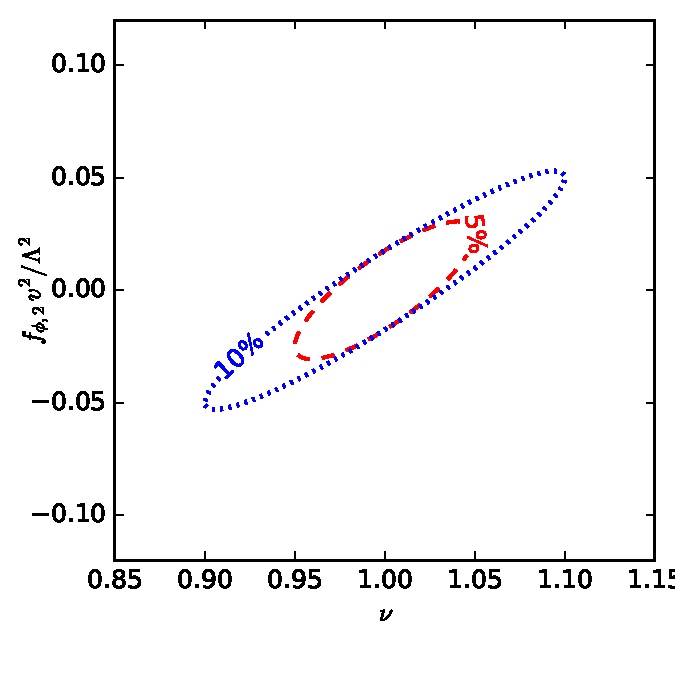
\includegraphics[height=0.45 \textwidth]{fig/information/wbf_tautau_systematics_nuisance.pdf}%
  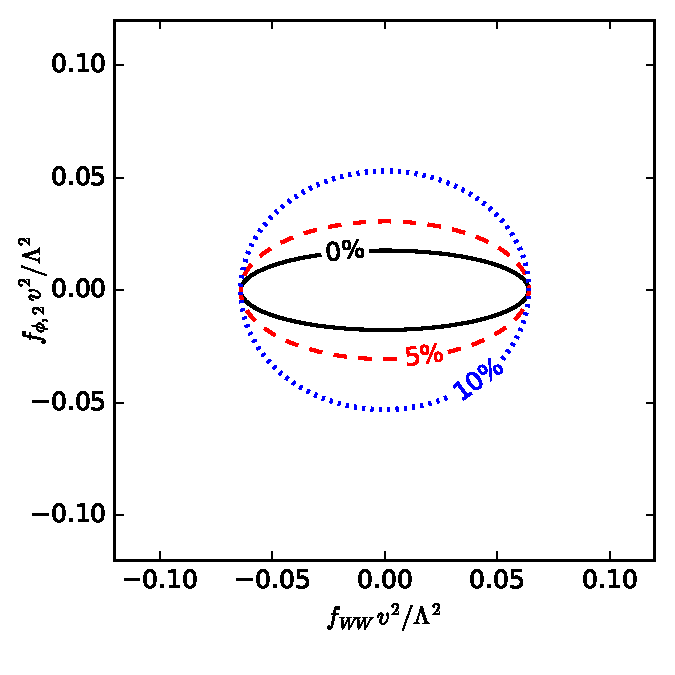
\includegraphics[height=0.45 \textwidth]{fig/information/wbf_tautau_systematics_profiled.pdf}%
  \caption{Effects of Gaussian uncertainties of $5\%$ and $10\%$ on
    the total signal rate. In the left panel we show the expected
    error ellipse $d_{\text{local}}( (g,\nu) ; \boldzero) = 1$ in
    the plane spanned by a physical parameter and the nuisance
    parameter $\nu$ rescaling the signal rate. In the right panel we
    show the error ellipses in the $\ope{W}$-$\ope{\phi,2}$ plane
    after profiling over this systematic uncertainty.}
  \label{fig:information_wbf_tautau_systematics}
\end{figure}

\begin{figure}
  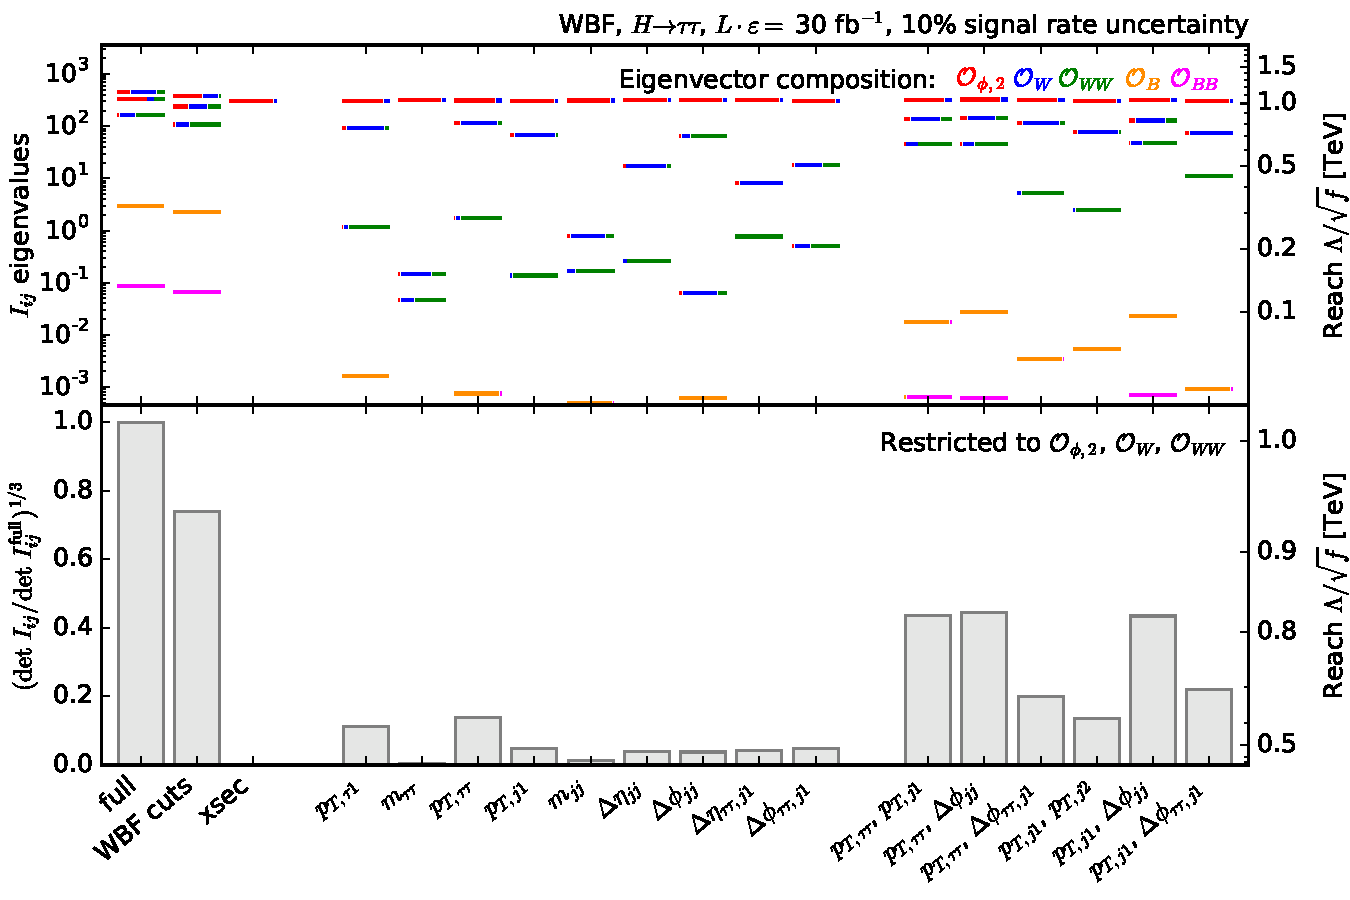
\includegraphics[height=0.6 \textwidth]{fig/information/wbf_tautau_histos_comparison_systematics.pdf}
  \caption{Fisher information for the WBF $H \to \tau \tau$ channel
    profiled over a $10\%$ signal rate uncertainty. We compare the
    information for the full phase space, after the cuts in
    \autoref{eq:wbf_tautau_wbfcuts}, and for several kinematic
    distributions.  The top panel shows the eigenvalues, the colors
    denote the composition of the corresponding eigenvectors. The
    right axis translates the eigenvalues into a new physics reach for
    the corresponding combination of Wilson coefficients.  In the
    bottom panel we show the determinants of the Fisher information
    restricted to $\ope{\phi,2}$, $\ope{W}$, and $\ope{WW}$,
    normalized to the full information. Again, the right axis
    translates them into a new physics reach.}
  \label{fig:information_wbf_tautau_systematics_comparison}
\end{figure}

We demonstrate this for WBF Higgs production in the $\tau \tau$ mode
in \autoref{fig:wbf_tautau_systematics}. We assign a $5\%$ or $10\%$
Gaussian uncertainty on the overall signal rate, representing for
instance missing higher orders, pdf or efficiency uncertainties. This
significantly reduces the information in the total rate, and thus
mostly the expected precision in the $\ope{\phi,2}$ direction.  In
\autoref{fig:wbf_tautau_systematics_comparison} we show how the
information in various distributions is affected by such an
uncertainty. The new physics reach in the $\ope{\phi,2}$ direction is
reduced by 800~GeV. 




%%%%%%%%%%%%%%%%%%%%%%%%%%%%%%%%%%%%%%%%%%%%%%%%%%%%%%%%%%%%
\subsection{Comparison with other tools}
%%%%%%%%%%%%%%%%%%%%%%%%%%%%%%%%%%%%%%%%%%%%%%%%%%%%%%%%%%%%

%%%%%%%%%%%%%%%%%%%%%%%%%%%%%%%%%%%%%%%%%%%%%%%%%%%%%%%%%%%%
\subsubsection*{Likelihood ratio}
%%%%%%%%%%%%%%%%%%%%%%%%%%%%%%%%%%%%%%%%%%%%%%%%%%%%%%%%%%%%

There is some subtlety in the relationship between 
standard likelihood ratio tests and the Fisher distance.
We anticipate that the confidence intervals in $\boldtheta$ will continue 
to be based on likelihood ratio tests.
While both are invariant to reparametrization of $\boldtheta$, 
 non-linear terms in $\boldtheta$ that lead to curvature in the information
geometry can break the one-to-one relationship between the 
expected value of the log-likelihood ratio and the Fisher information distance.

In \autoref{fig:wbf_tautau_llr} we compare the two tools. As an
example, we study WBF Higgs production in the $\tau \tau$ mode and
sample parameter points $\boldtheta$ in the $\ope{W}$-$\ope{WW}$
plane. For each of these points we calculate the local and global
distance from the SM defined by the Fisher information, as well as the
expected log-likelihood ratio 
%
\begin{align}
  q(\boldtheta_b , \boldtheta_a )
  \equiv -2 \, E \left[
  \log \frac { f(\mathbf{x}|\boldtheta_b) }   { f(\mathbf{x} |\boldtheta_a) }
  \middle | \boldtheta_a \right] \,.
\end{align}
%
For small significance deviations, the local and especially the global distances are 
almost exactly equal to the expected likelihood ratio, 
with differences only becoming visible around the $3 \sigma$ level. 
This demonstrates that different
statistical tools probe the same physics and can be chosen based on
convenience.

\begin{figure}
  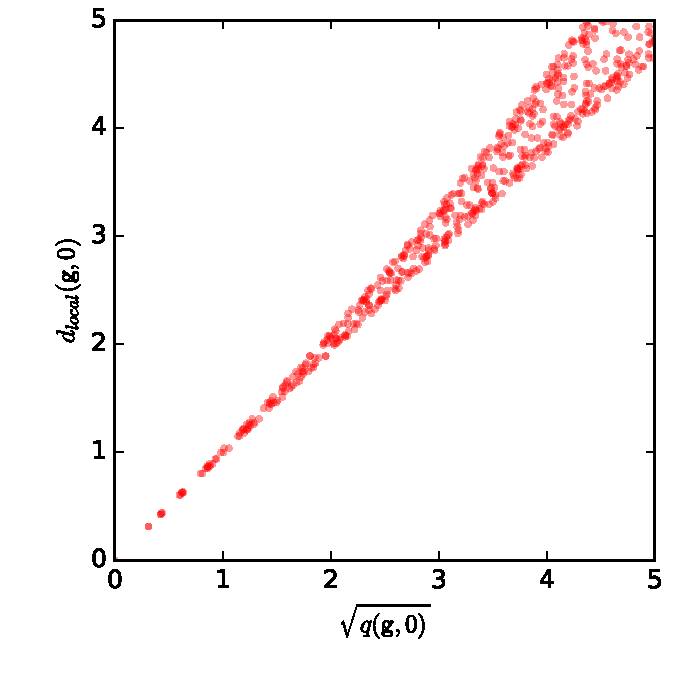
\includegraphics[height=0.45 \textwidth]{fig/information/wbf_tautau_local_distance_vs_llr}
  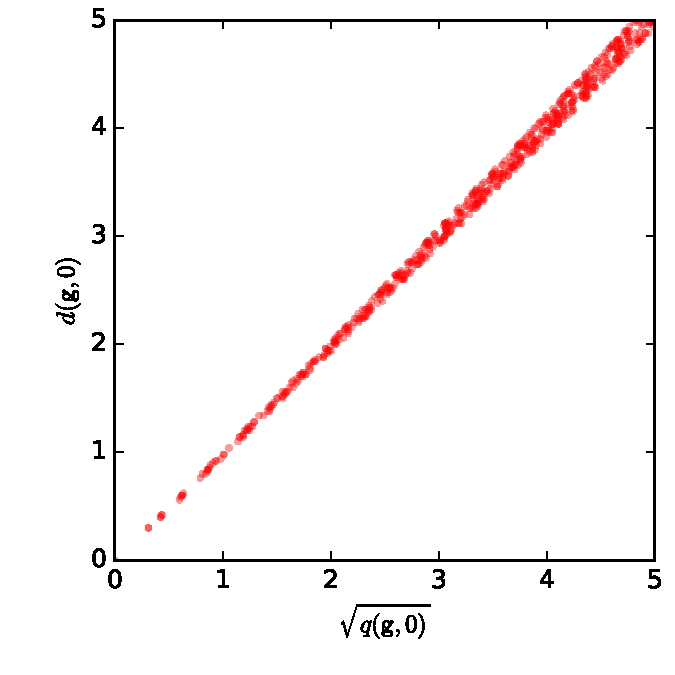
\includegraphics[height=0.45 \textwidth]{fig/information/wbf_tautau_distance_vs_llr}
  \caption{Comparison of the local (left) and global (right) distances
    defined by the Fisher information with the expected local
    likelihood ratio. We use WBF Higgs production in the $\tau \tau$
    mode and sample parameter points in the $\ope{W}$-$\ope{WW}$
    plane.}
  \label{fig:information_wbf_tautau_llr}
\end{figure}



%%%%%%%%%%%%%%%%%%%%%%%%%%%%%%%%%%%%%%%%%%%%%%%%%%%%%%%%%%%%
\subsubsection*{Ambient geometry}
%%%%%%%%%%%%%%%%%%%%%%%%%%%%%%%%%%%%%%%%%%%%%%%%%%%%%%%%%%%%




%%%%%%%%%%%%%%%%%%%%%%%%%%%%%%%%%%%%%%%%%%%%%%%%%%%%%%%%%%%%
\section{Conclusions}
\label{sec:information_conclusions}
%%%%%%%%%%%%%%%%%%%%%%%%%%%%%%%%%%%%%%%%%%%%%%%%%%%%%%%%%%%%

We have used information geometry to calculate the maximum sensitivity
of Higgs measurements to dimension-6 operators, to understand the
structure of the observables, and to discuss how to improve these
measurements. Our approach is based on the Fisher information matrix,
which according to the Cram\'er-Rao bound defines the maximum
precision that can be achieved in a measurement. Unlike traditional
multivariate analysis techniques, it is designed for continuous,
high-dimensional parameter spaces like effective field theories. We
have demonstrated how the Fisher information can be reliably
calculated using Monte-Carlo techniques.

Going beyond global statements, the Fisher information can be studied
differentially to understand how the discriminating power is
distributed over phase space, which helps guide event selection
strategies.  Moreover, we can also calculate the information contained
in a subsets of kinematic distributions. This helps us determine
which observables are the most powerful, and allows us to compare the
constraining power in conventional analyses with one or two variables
to that in more complex multivariate analyses.

Our first testing ground was Higgs production in weak boson fusion
with decays into a tau pair or into four leptons. Crucial information
comes from the high-energy tails as well as from angular correlations
between jets. Decay kinematics hardly adds any information, since the
momentum flow is limited by the Higgs mass and gauge invariance forces
us to include operators with a momentum dependence.  Tight cuts on the
rapidity separation of the tagging jets throw away a large amount of
discrimination power. Under idealized conditions, conventional
analyses based on a simple event selection and standard kinematic
distributions can probe new physics scales around $900~\gev$ in the
early phase of Run~II. Multivariate analyses have the potential to
significantly enhance the sensitivity and probe new physics scales of
up to $1.2~\tev$.

In Higgs production with a single top we find that kinematic
properties of the Higgs decay products and observables in the top
system provide orthogonal information. The transverse momenta of the
di-photon system as well as the rapidity separation of the
$\gamma \gamma$ and $bjj$ systems are powerful observables. But even
with HL-LHC data these distributions are only sensitive to new physics
scales around $550~\gev$, while a multivariate analysis might be able
to probe scales up to $700~\gev$.

To summarize, information geometry provides a powerful and intuitive
tool that can help understand the phenomenology of models with a
continuous, high-dimensional parameter space, and in turn can be used
to optimize measurement strategies.  We have demonstrated this
approach in different Higgs channels for dimension-6 operators, but
it can easily be translated to other processes and models.
